%%%%%%%%%%%%%%%%%%%%%%%%%%%%%%%%%%%%%%%%
% datoteka diploma-vzorec.tex
%
% vzorčna datoteka za pisanje diplomskega dela v formatu LaTeX
% na UL Fakulteti za računalništvo in informatiko
%
% vkup spravil Gašper Fijavž, december 2010
% 
%
%
% verzija 12. februar 2014 (besedilo teme, seznam kratic, popravki Gašper Fijavž)
% verzija 10. marec 2014 (redakcijski popravki Zoran Bosnić)
% verzija 11. marec 2014 (redakcijski popravki Gašper Fijavž)
% verzija 15. april 2014 (pdf/a 1b compliance, not really - just claiming, Damjan Cvetan, Gašper Fijavž)
% verzija 23. april 2014 (privzeto cc licenca)
% verzija 16. september 2014 (odmiki strain od roba)
% verzija 28. oktober 2014 (odstranil vpisno številko)
% verija 5. februar 2015 (Literatura v kazalu, online literatura)
% verzija 25. september 2015 (angl. naslov v izjavi o avtorstvu)
% verzija 26. februar 2016 (UL izjava o avtorstvu)
% verzija 16. april 2016 (odstranjena izjava o avtorstvu)
% verzija 5. junij 2016 (Franc Solina dodal vrstice, ki jih je označil s svojim imenom)


\documentclass[a4paper, 12pt]{book}
%\documentclass[a4paper, 12pt, draft]{book}  Nalogo preverite tudi z opcijo draft, ki vam bo pokazala, katere vrstice so predolge!



\usepackage[utf8x]{inputenc}   % omogoča uporabo slovenskih črk kodiranih v formatu UTF-8
\usepackage[slovene,english]{babel}    % naloži, med drugim, slovenske delilne vzorce
\usepackage[pdftex]{graphicx}  % omogoča vlaganje slik različnih formatov
\usepackage{fancyhdr}          % poskrbi, na primer, za glave strani
\usepackage{amssymb}           % dodatni simboli
\usepackage{amsmath}           % eqref, npr.
%\usepackage{hyperxmp}
\usepackage[hyphens]{url}  % dodal Solina
\usepackage{comment}       % dodal Solina

\usepackage[pdftex, colorlinks=true,
						citecolor=black, filecolor=black, 
						linkcolor=black, urlcolor=black,
						pagebackref=false, 
						pdfproducer={LaTeX}, pdfcreator={LaTeX}, hidelinks]{hyperref}

\usepackage{color}       % dodal Solina
\usepackage{soul}       % dodal Solina

%%%%%%%%%%%%%%%%%%%%%%%%%%%%%%%%%%%%%%%%
%	DIPLOMA INFO
%%%%%%%%%%%%%%%%%%%%%%%%%%%%%%%%%%%%%%%%
\newcommand{\ttitle}{Učenje realno-časovne strateške igre z uporabo globokega spodbujevalnega učenja}
\newcommand{\ttitleEn}{Learning a real-time strategy game with deep reinforcement learning}
\newcommand{\tsubject}{\ttitle}
\newcommand{\tsubjectEn}{\ttitleEn}
\newcommand{\tauthor}{Jernej Habjan}
\newcommand{\tkeywords}{AlphaZero, realno-časovna strateška igra, Unreal Engine}
\newcommand{\tkeywordsEn}{AlphaZero, real-time strategy game, Unreal Engine}


%%%%%%%%%%%%%%%%%%%%%%%%%%%%%%%%%%%%%%%%
%	HYPERREF SETUP
%%%%%%%%%%%%%%%%%%%%%%%%%%%%%%%%%%%%%%%%
\hypersetup{pdftitle={\ttitle}}
\hypersetup{pdfsubject=\ttitleEn}
\hypersetup{pdfauthor={\tauthor, jh0228@student.uni-lj.si}}
\hypersetup{pdfkeywords=\tkeywordsEn}

%%%%%%%%%%%%%%%%%%%%%%%%%%%%%%%%%%%%%%%%
% postavitev strani
%%%%%%%%%%%%%%%%%%%%%%%%%%%%%%%%%%%%%%%%  

\addtolength{\marginparwidth}{-20pt} % robovi za tisk
\addtolength{\oddsidemargin}{40pt}
\addtolength{\evensidemargin}{-40pt}

\renewcommand{\baselinestretch}{1.3} % ustrezen razmik med vrsticami
\setlength{\headheight}{15pt}        % potreben prostor na vrhu
\renewcommand{\chaptermark}[1]%
{\markboth{\MakeUppercase{\thechapter.\ #1}}{}} \renewcommand{\sectionmark}[1]%
{\markright{\MakeUppercase{\thesection.\ #1}}} \renewcommand{\headrulewidth}{0.5pt} \renewcommand{\footrulewidth}{0pt}
\fancyhf{}
\fancyhead[LE,RO]{\sl \thepage} 
%\fancyhead[LO]{\sl \rightmark} \fancyhead[RE]{\sl \leftmark}
\fancyhead[RE]{\sc \tauthor}              % dodal Solina
\fancyhead[LO]{\sc Diplomska naloga}     % dodal Solina


\newcommand{\BibTeX}{{\sc Bib}\TeX}

%%%%%%%%%%%%%%%%%%%%%%%%%%%%%%%%%%%%%%%%
% naslovi
%%%%%%%%%%%%%%%%%%%%%%%%%%%%%%%%%%%%%%%%  


\newcommand{\autfont}{\Large}
\newcommand{\titfont}{\LARGE\bf}
\newcommand{\clearemptydoublepage}{\newpage{\pagestyle{empty}\cleardoublepage}}
\setcounter{tocdepth}{1}	      % globina kazala

%%%%%%%%%%%%%%%%%%%%%%%%%%%%%%%%%%%%%%%%
% konstrukti
%%%%%%%%%%%%%%%%%%%%%%%%%%%%%%%%%%%%%%%%  
\newtheorem{izrek}{Izrek}[chapter]
\newtheorem{trditev}{Trditev}[izrek]
\newenvironment{dokaz}{\emph{Dokaz.}\ }{\hspace{\fill}{$\Box$}}

%%%%%%%%%%%%%%%%%%%%%%%%%%%%%%%%%%%%%%%%%%%%%%%%%%%%%%%%%%%%%%%%%%%%%%%%%%%%%%%
%% PDF-A
%%%%%%%%%%%%%%%%%%%%%%%%%%%%%%%%%%%%%%%%%%%%%%%%%%%%%%%%%%%%%%%%%%%%%%%%%%%%%%%


%%%%%%%%%%%%%%%%%%%%%%%%%%%%%%%%%%%%%%%% 
% define medatata
%%%%%%%%%%%%%%%%%%%%%%%%%%%%%%%%%%%%%%%% 
\def\Title{\ttitle}
\def\Author{\tauthor, jh0228@student.uni-lj.si}
\def\Subject{\ttitleEn}
\def\Keywords{\tkeywordsEn}

%%%%%%%%%%%%%%%%%%%%%%%%%%%%%%%%%%%%%%%% 
% \convertDate converts D:20080419103507+02'00' to 2008-04-19T10:35:07+02:00
%%%%%%%%%%%%%%%%%%%%%%%%%%%%%%%%%%%%%%%% 
\def\convertDate{%
    \getYear
}

{\catcode`\D=12
 \gdef\getYear D:#1#2#3#4{\edef\xYear{#1#2#3#4}\getMonth}
}
\def\getMonth#1#2{\edef\xMonth{#1#2}\getDay}
\def\getDay#1#2{\edef\xDay{#1#2}\getHour}
\def\getHour#1#2{\edef\xHour{#1#2}\getMin}
\def\getMin#1#2{\edef\xMin{#1#2}\getSec}
\def\getSec#1#2{\edef\xSec{#1#2}\getTZh}
\def\getTZh +#1#2{\edef\xTZh{#1#2}\getTZm}
\def\getTZm '#1#2'{%
    \edef\xTZm{#1#2}%
    \edef\convDate{\xYear-\xMonth-\xDay T\xHour:\xMin:\xSec+\xTZh:\xTZm}%
}

\expandafter\convertDate\pdfcreationdate 

%%%%%%%%%%%%%%%%%%%%%%%%%%%%%%%%%%%%%%%%
% get pdftex version string
%%%%%%%%%%%%%%%%%%%%%%%%%%%%%%%%%%%%%%%% 
\newcount\countA
\countA=\pdftexversion
\advance \countA by -100
\def\pdftexVersionStr{pdfTeX-1.\the\countA.\pdftexrevision}


%%%%%%%%%%%%%%%%%%%%%%%%%%%%%%%%%%%%%%%%
% XMP data
%%%%%%%%%%%%%%%%%%%%%%%%%%%%%%%%%%%%%%%%  
\usepackage{xmpincl}
\includexmp{pdfa-1b}

%%%%%%%%%%%%%%%%%%%%%%%%%%%%%%%%%%%%%%%%
% pdfInfo
%%%%%%%%%%%%%%%%%%%%%%%%%%%%%%%%%%%%%%%%  
\pdfinfo{%
    /Title    (\ttitle)
    /Author   (\tauthor, damjan@cvetan.si)
    /Subject  (\ttitleEn)
    /Keywords (\tkeywordsEn)
    /ModDate  (\pdfcreationdate)
    /Trapped  /False
}


%%%%%%%%%%%%%%%%%%%%%%%%%%%%%%%%%%%%%%%%%%%%%%%%%%%%%%%%%%%%%%%%%%%%%%%%%%%%%%%
%%%%%%%%%%%%%%%%%%%%%%%%%%%%%%%%%%%%%%%%%%%%%%%%%%%%%%%%%%%%%%%%%%%%%%%%%%%%%%%

\begin{document}
\selectlanguage{slovene}
\frontmatter
\setcounter{page}{1} %
\renewcommand{\thepage}{}       % preprecimo težave s številkami strani v kazalu
\newcommand{\sn}[1]{"`#1"'}                    % dodal Solina (slovenski narekovaji)

%%%%%%%%%%%%%%%%%%%%%%%%%%%%%%%%%%%%%%%%
%naslovnica
 \thispagestyle{empty}%
   \begin{center}
    {\large\sc Univerza v Ljubljani\\%
      Fakulteta za računalništvo in informatiko}%
    \vskip 10em%
    {\autfont \tauthor\par}%
    {\titfont \ttitle \par}%
    {\vskip 3em \textsc{DIPLOMSKO DELO\\[5mm]         % dodal Solina za ostale študijske programe
%    VISOKOŠOLSKI STROKOVNI ŠTUDIJSKI PROGRAM\\ PRVE STOPNJE\\ RAČUNALNIŠTVO IN INFORMATIKA}\par}%
    UNIVERZITETNI  ŠTUDIJSKI PROGRAM\\ PRVE STOPNJE\\ RAČUNALNIŠTVO IN INFORMATIKA}\par}%
%    INTERDISCIPLINARNI UNIVERZITETNI\\ ŠTUDIJSKI PROGRAM PRVE STOPNJE\\ RAČUNALNIŠTVO IN MATEMATIKA}\par}%
%    INTERDISCIPLINARNI UNIVERZITETNI\\ ŠTUDIJSKI PROGRAM PRVE STOPNJE\\ UPRAVNA INFORMATIKA}\par}%
%    INTERDISCIPLINARNI UNIVERZITETNI\\ ŠTUDIJSKI PROGRAM PRVE STOPNJE\\ MULTIMEDIJA}\par}%
    \vfill\null%
    {\large \textsc{Mentor}: doc.\ dr. Matej Guid\par}%
   {\large \textsc{Somentor}:  prof.\ dr. Branko Šter \par}%
    {\vskip 2em \large Ljubljana, 2018 \par}%
\end{center}
% prazna stran
%\clearemptydoublepage      % dodal Solina (izjava o licencah itd. se izpiše na hrbtni strani naslovnice)

%%%%%%%%%%%%%%%%%%%%%%%%%%%%%%%%%%%%%%%%
%copyright stran
\thispagestyle{empty}
\vspace*{8cm}

\noindent
{\sc Copyright}. 
Rezultati diplomske naloge so intelektualna lastnina avtorja in Fakultete za računalništvo in informatiko Univerze v Ljubljani.
Za objavo in koriščenje rezultatov diplomske naloge je potrebno pisno privoljenje avtorja, Fakultete za računalništvo in informatiko ter mentorja.

\begin{center}
\mbox{}\vfill
\emph{Besedilo je oblikovano z urejevalnikom besedil \LaTeX.}
\end{center}
% prazna stran
\clearemptydoublepage

%%%%%%%%%%%%%%%%%%%%%%%%%%%%%%%%%%%%%%%%
% stran 3 med uvodnimi listi
\thispagestyle{empty}
\vspace*{4cm}

\noindent
Fakulteta za računalništvo in informatiko izdaja naslednjo nalogo:
\medskip
\begin{tabbing}
\hspace{32mm}\= \hspace{6cm} \= \kill
Tematika naloge:
\end{tabbing}
Besedilo teme diplomskega dela študent prepiše iz študijskega informacijskega sistema, kamor ga je vnesel mentor. V nekaj stavkih bo opisal, kaj pričakuje od kandidatovega diplomskega dela. Kaj so cilji, kakšne metode uporabiti, morda bo zapisal tudi ključno literaturo.
\vspace{15mm}
\vspace{2cm}
% prazna stran
\clearemptydoublepage
% zahvala
\thispagestyle{empty}\mbox{}\vfill\null\it%
\noindent
Zahvaljujem se mentorju doc.\ dr. Mateju Guidu in somentorju prof.\ dr. Branku Šteru, prijateljem in družini, ki so mi pomagali pri pisanju diplomske naloge.
\rm\normalfont
% prazna stran
\clearemptydoublepage
% kazalo
\pagestyle{empty}
\def\thepage{}% preprecimo tezave s stevilkami strani v kazalu
\tableofcontents{}
% prazna stran
\clearemptydoublepage

%%%%%%%%%%%%%%%%%%%%%%%%%%%%%%%%%%%%%%%%
% seznam kratic

\chapter*{Seznam uporabljenih kratic}  % spremenil Solina, da predolge vrstice ne gredo preko desnega roba

\begin{comment}
\begin{tabular}{l|l|l}
  {\bf kratica} & {\bf angleško} & {\bf slovensko} \\ \hline
  % after \\: \hline or \cline{col1-col2} \cline{col3-col4} ...
  {\bf CA} & classification accuracy & klasifikacijska točnost \\
  {\bf DBMS} & database management system & sistem za upravljanje podatkovnih baz \\
  {\bf SVM} & support vector machine & metoda podpornih vektorjev \\
  \dots & \dots & \dots \\
\end{tabular}
\end{comment}

\noindent\begin{tabular}{p{0.1\textwidth}|p{.4\textwidth}|p{.4\textwidth}}    % po potrebi razširi prvo kolono tabele na račun drugih dveh!
	{\bf kratica} & {\bf angleško} & {\bf slovensko} \\ \hline
	{\bf MCTS} & Monte Carlo tree search & drevesno preiskovanje Monte Carlo \\
	{\bf UE4} & game engine Unreal Engine 4 & celostni pogon Unreal Engine 4 \\
	{\bf RTS} & real-time strategy & realno-časovna strateška\\
	{\bf One hot} & one hot & kodiranje z eno enico v zapisu vsakega stanja  \\
	{\bf JSON} & JavaScript Object Notation & notacija za označevanje JavaScript objektov \\
\end{tabular}


% prazna stran
\clearemptydoublepage

%%%%%%%%%%%%%%%%%%%%%%%%%%%%%%%%%%%%%%%%
% povzetek
\addcontentsline{toc}{chapter}{Povzetek}
\chapter*{Povzetek}

\noindent\textbf{Naslov:} \ttitle
\bigskip

\noindent\textbf{Avtor:} \tauthor
\bigskip

%\noindent\textbf{Povzetek:} 
\noindent 
Z obstoječim AlphaZero algoritmom smo implementirali učenje in priporočanje akcij v realno-časovni strateški igri.
Pregledali smo krajšo zgodovino globokega spodbujevalnega učenja na igrah in povzeli zakaj je pristop samostojnega učenja najprimernejši.
Za strateško igro smo določili figure in njihove akcije in zakodirali kompleksno stanje igre s kodirnikom.
Določili smo ustavitvene pogoje pri igri, ki nima končnega števila potez na podlagi zmanjšanja življenjskih točk figur.
Rezultate smo prikazali s Python modulom Pygame in v celostnem pogonu Unreal Engine 4. 
V obeh vizualizacijah lahko igramo proti naučenem modelu, ali opazujemo, kako se dva računalniška nasprotnika bojujeta med sabo.
Na koncu smo pregledali rezultate in povzeli učinek učenja algoritma.
\bigskip

\noindent\textbf{Ključne besede:} \tkeywords.
% prazna stran
\clearemptydoublepage

%%%%%%%%%%%%%%%%%%%%%%%%%%%%%%%%%%%%%%%%
% abstract
\selectlanguage{english}
\addcontentsline{toc}{chapter}{Abstract}
\chapter*{Abstract}

\noindent\textbf{Title:} \ttitleEn
\bigskip

\noindent\textbf{Author:} \tauthor
\bigskip

%\noindent\textbf{Abstract:} 
\noindent With the existing AlphaZero algorithm we have implemented the learning and recommendation of actions in a real-time strategy game.
We examined the shorter history of deep reinforcement learning in games and summarized why the self-learning approach is best suited.
For a strategic game we defined the characters and their actions and coded the complex state of the game with the encoder.
We have also determined the stop conditions of the game, which has no number of moves due to damage to the pieces.
The results were displayed with the Python Pygame module and the integrated drive of the Unreal Engine 4.
In both visualizations we can play against the learned model, or we can observe two computer opponents fighting against each other.
In the end, we also reviewed the results and summarized the learning effect of the algorithm.
\bigskip

\noindent\textbf{Keywords:} \tkeywordsEn.
\selectlanguage{slovene}
% prazna stran
\clearemptydoublepage

%%%%%%%%%%%%%%%%%%%%%%%%%%%%%%%%%%%%%%%%
\mainmatter
\setcounter{page}{1}
\pagestyle{fancy}


%%%%%%%%%%%%%%%%%%%%%%%%%%%%%%%%%%%%%%%%%%%%%%%%%%%%%%%%%%%%%%%%%%%%%%%%%%%%%%%%%%%%%%%%%%%%%%%%%%%%%%%%%%%%%%%%%%%%%%%%
%%%%%%%%%%%%%%%%%%%%%%%%%%%%%%%%%%%%%%%%%%%%%%%%%%%%%%%%%%%%%%%%%%%%%%%%%%%%%%%%%%%%%%%%%%%%%%%%%%%%%%%%%%%%%%%%%%%%%%%%
%%%%%%%%%%%%%%%%%%%%%%%%%%%%%%%%%%%%%%%%%%%%%%%%%%%%%%%%%%%%%%%%%%%%%%%%%%%%%%%%%%%%%%%%%%%%%%%%%%%%%%%%%%%%%%%%%%%%%%%%
%%%%%%%%%%%%%%%%%%%%%%%%%%%%%%%%%%%%%%%%%%%%%%%%%%%%%%%%%%%%%%%%%%%%%%%%%%%%%%%%%%%%%%%%%%%%%%%%%%%%%%%%%%%%%%%%%%%%%%%%
%%%%%%%%%%%%%%%%%%%%%%%%%%%%%%%%%%%%%%%%%%%%%%%%%%%%%%%%%%%%%%%%%%%%%%%%%%%%%%%%%%%%%%%%%%%%%%%%%%%%%%%%%%%%%%%%%%%%%%%%
\chapter{Uvod}


Razvijanje inteligentnega agenta v realno-časovnih strateških (ang. real-time strategy; RTS) igrah je problem, s katerim se mora soočiti večina razvijalcev teh iger. 
Agentove akcije so vnaprej kodiranje in so zato pogosto predvidljive, saj se človeški igralec nauči njihovih načinov delovanja in jih tako lažje premaga.
Če pustimo agentu, da sam opravlja akcije nekontrolirano, bo te akcije izvajal naključno, ki so večino časa slabše kot vnaprej opisana taktika.
Agentu lahko podamo hevristiko, ki predstavlja pravilo po katerem mora delovati da doseže boljšo performanco.
Ta se po njej ravna in z njeno pomočjo poskuša izvesti čim boljšo akcijo, vendar bo za njen izračun porabil dolgo časa, saj bo moral pregledati cel preiskovalni prostor, ki je pri realno-časovnih strateških igrah prevelik.
Na primer 10 figur v igri, kjer ima vsaka 5 možnih potez, se razveji na možen faktor $5^{10}$ ≈ 10 milijonov možnih akcij.
Za realno-časovno strateško igro StarCraft je ocenjenih možnih vsaj $10^{1685}$ možnih akcij, kjer je za šah ponavadi ocenjeno med $10^{40}$ in $10^{50}$, natančneje $\dfrac{64!}{32!8!^{2}2!^{6}}$, kar je približno $10^{43}$~\cite{wiki:Shannon_number} ter faktor vejanja $10^{171}$ pri igro Go~\cite{ontanon2017combinatorial}.
Za primerjavo lahko kot zanimivost vzamemo število atomov v opazovanem vesolju, ki obsega med $10^{78}$ in $10^{82}$~\cite{atoms}.

Preiskovanje prostora z grobo silo torej odpade. 
Ostanejo nam potem hevristični algoritmi, kot na primer Alpha-Beta rezanje ali drevesno preiskovanje Monte Carlo (ang. Monte Carlo tree search; MCTS). 
Seveda pa moramo upoštevati, da algoritem Alpha-Beta rezanje deluje dobro samo pod pogoji, da obstaja zanesljiva ocenitvena funkcija in da ima igra majhen vejitveni prostor, kar je pa v nasprotju z veliko klasičnimi namiznimi igrami kot npr. igra Go in video igrami. 
Zato se je v takšnih primerih bolje odločiti za algoritem MCTS~\cite{chaslot2008monte}.
Ta ima pomanjkljivost, da si stanj igre ne zapomni skozi iteracij več iger, kjer bi lahko to vrednost stanja uporabil za bolj natančen izračun naslednjih stanj.

Za pomnjenje stanj so primerne globoke nevronske mreže, ki z učenjem ugotovijo zakonitosti v učni množici in skozi mnogo iteracij učenja izboljšajo svojo napoved določenega izhoda ob določenem vhodu. 
To je točno to, kar potrebuje MCTS kot začetno stanje, iz katerega lažje izračunamo najboljšo akcijo.

Da nevronska mreža dobi dovolj vhodnih podatkov za učenje, moramo realizirati algoritem, ki bo igral proti drugem računalniškem nasprotniku.
S tem bo algoritem izgradil dovolj veliko učno množico z rezultati zmag oziroma porazov teh iger. 
Ob tem nevronska mreža posodobi svojo napoved akcij za določeno stanje igre, kar v prihodnosti pomeni boljšo napoved akcije.

To je glavna ideja o implementaciji algoritma, ki jo vsebuje algoritem AlphaZero, ki smo ga uporabili v naši diplomski nalogi.
Algoritem se lahko uporabi tudi za učenje igranja raznih namiznih iger, realno-časovnih strateških iger z igranjem mnogo iger sam proti sebi (boljša različica algoritma napreduje v naslednjo iteracijo).
Ko je model nevronske mreže naučen, ga lahko uporabimo, da nam priporoči akcijo v določenem stanju.
S tem lahko implementiramo računalniškega igralca, ki pridobiva priporočene akcije od naučenega modela in jih izvršuje, kot tudi priporočilni sistem za akcije, ki jih prikazujemo človeškemu igralcu kot pomoč oziroma učenje človeškega igralca igranja igre. 
Algoritem nam priporoči akcijo in ne strategije (za to bi potrebovali bolj abstrakten pogled na igro). 

O strateških igrah, njihovih abstrakcijah in zakaj so tako zanimive za raziskovanje na področju umetne inteligence bomo več spoznali v poglavju~\ref{chrts}.
Za tem si bomo podrobneje pregledali sestavo AlphaZero algoritma in zakaj je primeren za našo realno-časovno strateško igro v poglavju~\ref{alphazero}.
Ko bomo imeli izdelan algoritem učenja, bomo zanj sestavili RTS igro v poglavju~\ref{chpravilaigre} in izpostavili, kaj so glavne težave pri teh igrah v zvezi z njihovim učenjem.
Algoritem bomo na novo opisani igri naučili v poglavju~\ref{chucenjemodela}, kjer bomo pregledali razne parametre učenja in model potem preizkusili z vizualizacijo v Python modulu Pygame in celostnem pogonu Unreal Engine 4 v poglavju~\ref{chvizualizacija}.
Rezultate učenja bomo v poglavju~\ref{chrezultati} ocenili in ugotovili, katera vrsta učnih parametrov nam je podala najboljši rezultat.
V poglavju~\ref{chdiskusija} bomo rezultate pregledali s širše perspektive, omenili bomo tudi možne nadaljnje pristope in izboljšave, ki bi pomagale pri učenju algoritma. 
Pregledali bomo tudi koristnost aplikacije naučenega modela v pogon kot je Unreal Engine in kaj so njegove omejitve.
Na koncu bomo v poglavju~\ref{chzakljucek} naredili kratek pregled dosežkov in prispevkov diplomske naloge.

%%%%%%%%%%%%%%%%%%%%%%%%%%%%%%%%%%%%%%%%%%%%%%%%%%%%%%%%%%%%%%%%%%%%%%%%%%%%%%%%%%%%%%%%%%%%%%%%%%%%%%%%%%%%%%%%%%%%%%%%
%%%%%%%%%%%%%%%%%%%%%%%%%%%%%%%%%%%%%%%%%%%%%%%%%%%%%%%%%%%%%%%%%%%%%%%%%%%%%%%%%%%%%%%%%%%%%%%%%%%%%%%%%%%%%%%%%%%%%%%%
%%%%%%%%%%%%%%%%%%%%%%%%%%%%%%%%%%%%%%%%%%%%%%%%%%%%%%%%%%%%%%%%%%%%%%%%%%%%%%%%%%%%%%%%%%%%%%%%%%%%%%%%%%%%%%%%%%%%%%%%
%%%%%%%%%%%%%%%%%%%%%%%%%%%%%%%%%%%%%%%%%%%%%%%%%%%%%%%%%%%%%%%%%%%%%%%%%%%%%%%%%%%%%%%%%%%%%%%%%%%%%%%%%%%%%%%%%%%%%%%%
%%%%%%%%%%%%%%%%%%%%%%%%%%%%%%%%%%%%%%%%%%%%%%%%%%%%%%%%%%%%%%%%%%%%%%%%%%%%%%%%%%%%%%%%%%%%%%%%%%%%%%%%%%%%%%%%%%%%%%%%

\chapter{Realno-časovne strateške igre}
\label{chrts}

Realno-časovne strateške igre so žanr strateških iger, kjer igralec nadzoruje množico figur, in poskuša premagati nasprotnika z izgradnjo ekonomije, izboljšavo raznih tehnologij in urjenjem primernih vojaških figur, ki dodajo dodano vrednost h končnem cilju poraza nasprotnega igralca in s tem zmagi igre.
Igre se odvijajo v realnem času, kar pomeni da se stanje igre lahko spremeni večkrat na sekundo in s tem igralca prisili k stalnem fokusu na igro.
Primer RTS igre sta igra Age of Empires II (Ensemble Studios) in igra StarCraft (Blizzard Entertainment, THQ)~\ref{picRtsGames}. 

\begin{figure}[h]
	\begin{center}
		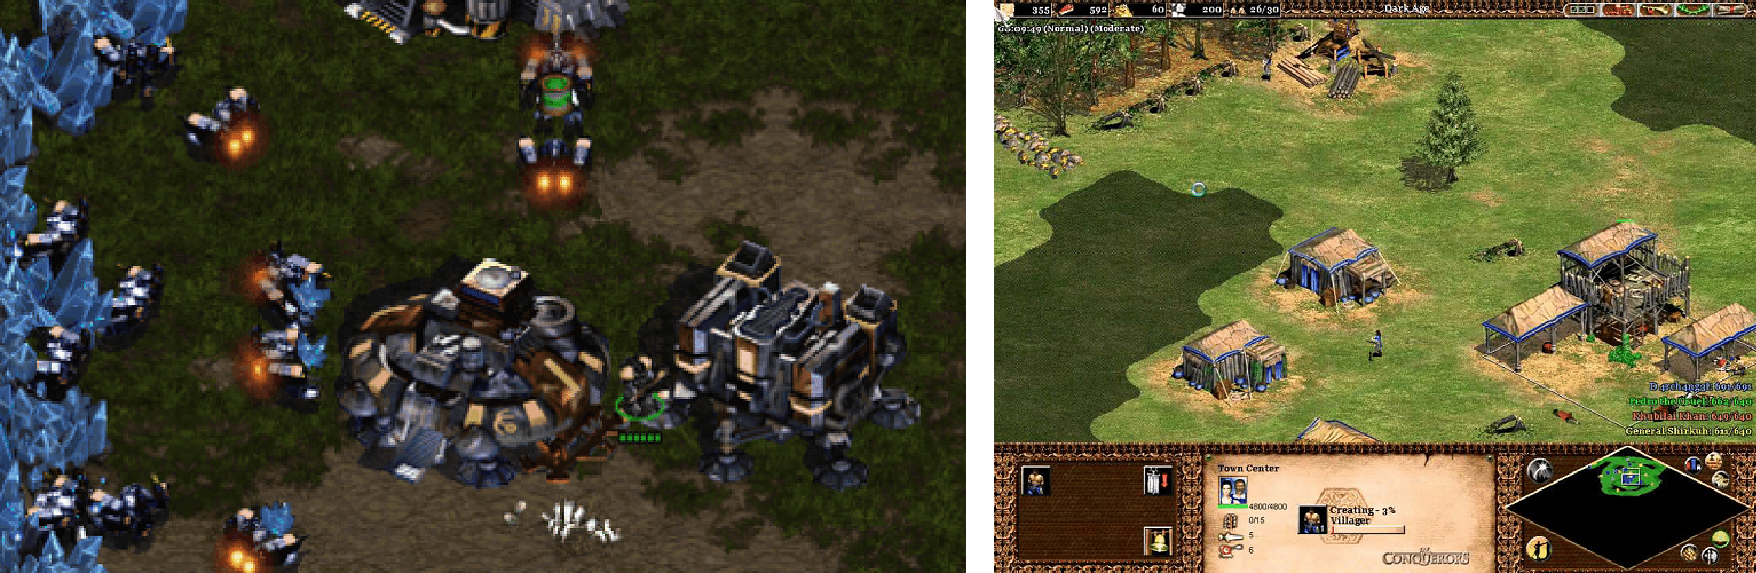
\includegraphics[width=1.0\textwidth]{photos/horizontal_rts.pdf}
	\end{center}
	\caption{Na zgornjih dveh slikah sta predstavljeni igra StarCraft (levo) in Age of Empires II (desno). Obe igri sta prikazani v začetnem stanju, kjer sta na slikah vidni glavni hiši, delavci, viri surovin (minerali, rude zlata, drevesa ipd.). Pri igri Age of Empires II je viden zemljevid, kjer zasenčenost predstavlja neraziskan del. Izvajanje določenih akcij poteka več časa, saj na primer delavci pri igri StarCraft vračajo minerale več časovnih enot, pri igri Age of Empiress II pa se gradi delavec več časovnih enot.}
	\label{picRtsGames}
\end{figure}


Razlike realno-časovnih iger v primerjavi s tradicionalnimi namiznimi igrami je dobro opisal Santiago Ontañon v raziskovalnem delu Pregled učenja umetne inteligence na realno-časovnih strateških igrah in tekmovanja v igri StarCraft~\cite{survey_real_time_strategy_ai_research_starcraft}.
Te razlike so naslednje:
\begin{itemize}
	\item izvajanje akcij v istem časovnem intervalu, ki lahko trajajo več časovnih intervalov,
	\item odločitev akcij v krajšem časovnem obdobju, saj za razliko od šaha, kjer ima igralec na voljo več minut za izbiro poteze, se v igri kot npr. StarCraft stanje igre zamenja 24-krat na sekundo,
	\item igre so lahko le vidne na področjih kjer je igralec že raziskal določeno področje in imajo nanj vpogled igralčeve figure,
	\item večina iger ni determinističnih, ampak imajo akcije možnost uspeha,
	\item kompleksnost raziskovalnega prostora je veliko večji.

\end{itemize}

Zaradi teh razlik so nastopili razni izzivi:

\begin{itemize}
	\item planiranje: realno-časovne strateške igre imajo običajno večji raziskovalni prostor od tradicionalnih namiznih iger, kar prepreči globje raziskovanje stanj iger. 
	Kot bomo pozneje pregledali, se igre zato abstrahirajo na več nivojev.
	Višji kot je nivo, bolj dolgoročni so cilji, kot na primer gradnja ekonomije, na nižjem nivoju pa so kratkotrajnejši cilji kot premik posamezne figure ipd.,
	\item učenje: učenje igranja igre lahko poteka na način predhodnega učenja, ki uporablja posnetke že odigranih iger in na način učenja v igri, ki uporablja spodbujevalno učenje in modeliranje nasprotnika,
	\item negotovost: negotovost nastane zaradi nevidnosti nasprotnikovih figur in njegovih potez v vsakem trenutku. 
	Ne moremo določiti, katero akcijo bo nasprotnik izvedel, zato je potrebna izgradnja drevesa, ki nam pove največjo verjetnost izbrane nasprotnikove akcije v določenem stanju igre,
	\item prostorsko in časovno razumevanje: prostorsko razumevanje je usmerjeno k postavljanju stavb in pozicijo vojske za obrambo in napad, med tem ko je časovno razumevanje usmerjeno k ugotavljanju časovne primernosti izdelave določenih figur, ki so primerne za izboljšavo igralčeve ekonomije, tehnološkega drevesa ali čas napada ipd.,
	\item izkoriščanje znanja domen: v tradicionalnih igrah kot npr. šah se lahko zanašamo na dobre ovrednotenske funkcije kot na primer algoritem alpha-beta rezanje in tabele za opis stanja konca igre, v realno-časovnih strateških igrah ni jasno kako lahko računalniški nasprotniki uporabijo domenska znanja iz posnetkov iger, zato se razvijalci tovrstnih iger bolj osredotočajo na izgradnjo več različnih taktik, med katerimi se računalniški nasprotnik na podlagi hevristike odloča.
	\item razdelitev nalog (prikazano na sliki~\ref{picRazdelitevNalog}): večje in zahtevnejše naloge so razdeljene na manjše, ki jih uvrščamo v več nivojev glede na abstrakcijo.
	\begin{itemize}
		\item strategija je najvišji nivo abstrakcije, ki zajema okrog 3 minutna planiranja in vse figure ki jih igralec nadzoruje, 
		\item taktika, ki je implementacija trenutne strategije (pozicija vojaških enot, stavb - 30 sekundno planiranje),
		\item reakcijska kontrola, ki je implementacija taktike ki je osredotočena na posamezno figuro,
		\item analiza terena, ki se osredotoča na strnjena območja in na višinsko prednost,
		\item pridobivanje znanja, s katerim pridobivamo informacije o taktiki nasprotnika.
	\end{itemize}

	\begin{figure}[h]
		\begin{center}
			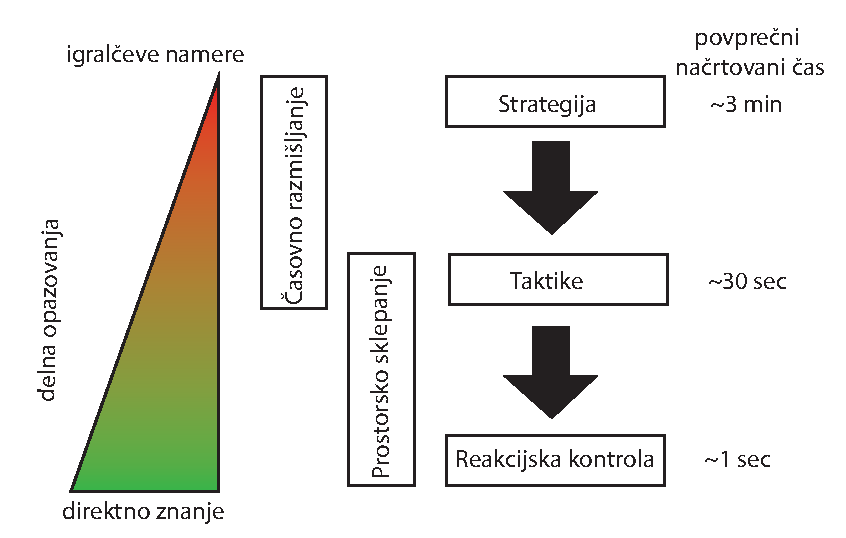
\includegraphics[width=0.8\textwidth]{photos/RazdelitevNalog.pdf}
		\end{center}
		\caption{Razdelitev nalog glede na čas reakcije in abstrakcije nalog. 
			Prikazani so nivoji odločanja glede na časovni razpon, kjer se negotovost akcij povečuje s povečevanjem ciljnega časa, za kar moramo igro pravilno abstrahirati na taktike in strategije. }
		\label{picRazdelitevNalog}
	\end{figure}

\end{itemize}

\section{Strategija}
V strateških igrah je velikokrat uporabljen pristop direktnega kodiranja strategije, ki uporabljajo avtomate končnih stanj, kjer lahko razbijemo delovanje na več stanj kot so napadanje, nabiranje surovin, popravilo itd. in hitro menjavanje med njimi. 
Direktno kodiranje prinese dobre pričakovane rezultate, vendar se lahko človeški igralec nauči te strategije in tako računalniškega agenta hitro porazi.
Planirani pristopi ponujajo večjo prilagodljivost kot direktno kodirani.
\section{Taktika}
Taktika spada pod neposrednejši nadzor figur kakor strategija in je bolj osredotočena na kontrolo določenih točk na mapi, zmagi posameznih bitk in iskanje ožin, kjer je nasprotnik šibkejši. 
Taktika temelji na analizi terena, ki ga lahko razbijemo na kompozicijo ožin.

\section{Abstrakcija prostora}

Razbiranje strategije in taktike je za algoritme umetne inteligence težja naloga od nadzorovanja posameznih figur, saj potrebuje višji nivo abstrakcije prostora, figur in akcij, kot za izbiro posameznih nizkonivojskih akcij.

Za primer abstrakcije prostora vzemimo računalniško realno-časovno igro, kjer bi lahko premik figure spremljali vsaka prikazana točka na prikazovalniku, vendar je primernejše da gledamo na premik figur kot izid na višjih ravneh abstrakcije igre~\cite{uriarte2015automatic}.
Posamezne figure vojaških enot lahko združujemo v večje skupine, katere potem obravnavamo in upravljamo kot en osebek.
Te skupine vojaških enot je potrebno pravilno razporediti na razne strateške točke, ki nam zagotavljajo znatno prednost pred nasprotnikom.
V ta namen lahko razgradimo zemljevid igre glede na ožine in prestope iz višjega na nižji del terena.
Na ta način lahko postavimo enote glede na novo razbiti teren~\cite{uriarte2014game}.
V našem delu smo zemljevid razbili kar na kvadratno mrežo 8x8 ali 6x6, saj ne vsebuje nobenih ožin in nedostopnih mest.
Imamo majhno število posameznih enot, ki lahko v računalniško igro apliciramo kot skupek enot, kot smo to opisali zgoraj.

Abstrakcija prostora poteka težje če igra vsebuje dejavnike negotovosti, kot na primer prekrivanje zemljevida z meglo (ang. Fog of war) kjer ne vidimo nasprotnikovih figur in potez v vsakem trenutku. 
Napoved nasprotnikovih potez je tako veliko težja, tako da vsi algoritmi s tako negotovostjo ne delujejo.
Mi smo se za diplomsko nalogo odločili, da imata oba računalniška agenta popoln vpogled na stanje igre in nasprotnikove akcije, saj je to privzeto delovanje izbranega algoritma AlphaZero.

V igri kot npr. StarCraft lahko posamezno vojaško enoto premaknemo na poljubno koordinato na zemljevidu, pod pogojem da je ta koordinata dosegljiva z vidika algoritma za iskanje poti.
Te koordinate premika lahko segajo tudi v neznane dele zemljevida, ki so lahko že zasedene z nasprotnikovo arhitekturo, zato lahko premikanje poenostavimo na sosednja polja.
Za napad nasprotnikovih enot, nabiranje zlatnikov ipd. lahko omejimo na izvajanje akcij znotraj določenega polja na najbližjo figuro.
Na primer vojaška enota lahko napade najbližjo nasprotnikovo enoto znotraj polja, v katerem je ta naša vojaška enota.
V našem primeru, kot bomo pojasnili pri poglavju opis pravil igre~\ref{chpravilaigre}, ne moremo postaviti več figur na isto polje, zato so akcije kot napad, nabiranje zlatnikov omejene na sosednja polja.

%%%%%%%%%%%%%%%%%%%%%%%%%%%%%%%%%%%%%%%%%%%%%%%%%%%%%%%%%%%%%%%%%%%%%%%%%%%%%%%%%%%%%%%%%%%%%%%%%%%%%%%%%%%%%%%%%%%%%%%%
%%%%%%%%%%%%%%%%%%%%%%%%%%%%%%%%%%%%%%%%%%%%%%%%%%%%%%%%%%%%%%%%%%%%%%%%%%%%%%%%%%%%%%%%%%%%%%%%%%%%%%%%%%%%%%%%%%%%%%%%
%%%%%%%%%%%%%%%%%%%%%%%%%%%%%%%%%%%%%%%%%%%%%%%%%%%%%%%%%%%%%%%%%%%%%%%%%%%%%%%%%%%%%%%%%%%%%%%%%%%%%%%%%%%%%%%%%%%%%%%%
%%%%%%%%%%%%%%%%%%%%%%%%%%%%%%%%%%%%%%%%%%%%%%%%%%%%%%%%%%%%%%%%%%%%%%%%%%%%%%%%%%%%%%%%%%%%%%%%%%%%%%%%%%%%%%%%%%%%%%%%
%%%%%%%%%%%%%%%%%%%%%%%%%%%%%%%%%%%%%%%%%%%%%%%%%%%%%%%%%%%%%%%%%%%%%%%%%%%%%%%%%%%%%%%%%%%%%%%%%%%%%%%%%%%%%%%%%%%%%%%%

\chapter{Predstavitev algoritma AlphaZero}
\label{alphazero}
\section{Zgodovina}

Igranje iger je popularno področje znotraj vede o umetni inteligenci. 
Desetletja je bil za raziskovalce s področja umetne inteligence podvig razviti program za igranje šaha.
Dandanes so najboljši algoritmi za igranje šaha nepremagljivi za celo svetovnega prvaka.
Ti algoritmi temeljijo na preiskovanju prostora več milijonov šahovskih pozicij in metodah, ki temeljijo na pravilih.
Za razliko od teh programov je bil eden izmed prvih programov programski pogon Checkers (Samuel 2000), ki se je naučil igranja z metodami samo-igranja in strojnega učenja in ne npr. na metodah ki temeljijo na pravilih.

Pri tradicionalnih namiznih igrah je faktor vejanja akcij relativno majhen in je lažje oceniti končno pozicijo iz danega stanja~\cite{wiki:AlphaGo}.
Rečeno je bilo, da igre kot npr. Go, ki imajo znatno večji faktor vejanja $10^{171}$ v primerjavi s šahom, ki ima $10^{47}$, ne bo možno ugotoviti vrednost končnega stanja še nekaj desetletij.
Algoritem AlphaGo~\cite{silver2016mastering} je naredil preboj s tem da uporablja metodo globokega spodbujevalnega učenja in algoritem drevesno preiskovanje Monte Carlo. 
Oktobra 2016 je premagal profesionalnega Go igralca na podlagi učenja na domenskem znanju iger, ki so jih odigrali eksperti.
Te sistemi so temeljili na predznanju ekspertov za učenje in ocenitev modela, kar pomeni, da ob igranju novih iger posnemajo katere akcije so eksperti izvajali ob določenem primeru.

Leto za tem, je bil razvit algoritem AlphaGo Zero~\cite{silver2017mastering}, ki opisuje pristop k učenju brez domenskega znanja ekspertov, ampak uporablja metodo samo-igranja~\ref{picCompareGo}. 
Novi model je tudi premagal AlphaGo algoritem, kar predstavlja odlične rezultate z vidika, da AlphaGo Zero ne potrebuje človeško usmerjanje pri učenju.
Računalniki se lahko tako naučijo reševanje problema brez človeških ekspertov, ki pogostejše delajo napake zaradi utrujenosti ali površnosti in nimajo takojšnega vpogleda na celotno zbirko iger, kot na to imajo računalniki.

\begin{figure}[h]
	\begin{center}
		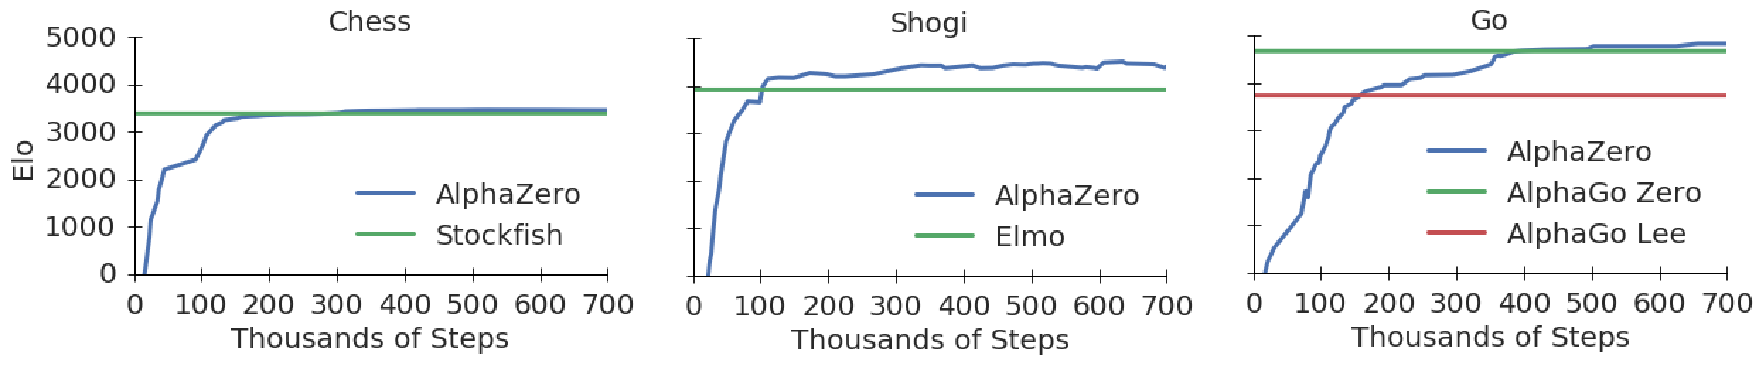
\includegraphics[width=1\textwidth]{photos/go.pdf}
	\end{center}
	\caption{Predstavitev igranja iger z naučenim algoritmom AlphaZero z 700,000 iteracijami, kjer je čas za napoved akcije je 1 sekunda. Na levi sliki je prikaz igranja šaha proti programu Stockfish iz leta 2016, na srednji sliki igranje proti programu Elmo iz leta 2017 v igri Shogi, na desni igranje igre Go proti proramoma AlphaGo Lee in AlphaGo Zero. }
	\label{picCompareGo}
\end{figure}

Delovanje algoritma AlphaGo Zero lahko opišemo v naslednjih korakih~\cite{guid}:
\begin{itemize}
	\item miselno odigraj igro z raziskovanjem neodkritega, pri čemer upoštevaj nasprotnikove akcije,
	\item pri soočenju z neznano pozicijo, oceni njeno vrednost in popravi ocene pozicij ki so vodile do trenutne pozicije,
	\item po prenehanju razmišljanja odigraj potezo ki je najbolj obetavna,
	\item po koncu igre preglej vse pozicije kjer si se za pozicije narobe odločil in jih popravi.
\end{itemize}


Za tem je bil razvit algoritem AlphaZero, ki vzame ideje AlphaGo Zero kot temelj, ampak je model generaliziran za poljubne igre, kot na primer šah, Shogi, Go, kjer algoritem potrebuje samo pravila igre, ta pa se uči igranja na podlagi globokih nevronskih mrež in tabula rasa algoritmom za spodbujevalno učenje.
Zaradi te generalizacije algoritma, lahko algoritem presliikamo na našo RTS igro, katero moramo sprva definirati da je kompatibilna z algoritmom.
Algoritem AlphaZero je drugačen od AlphaGo Zero v tem, da so igre pri AlphaGo Zero nastale z igranjem vseh posameznih modelov prejšnjih iteracij, na kar se je moč modela izračunala proti najboljšim igralcem, medtem ko AlphaZero samo hrani eno nevronsko mrežo, ki se stalno posodablja, namesto da čaka iteracijo da se konča.
\section{Potek učenja}
\label{potekUcenja}
AlphaZero se uči verjetnosti in ocenitve končnega stanja izključno z igranjem proti samemu sebi. 
Te potem uporabi pri preiskovanju z glavno namensko metodo drevesnim preiskovanjem Monte Carlo, da razišče drevo stanj za akcijo.
Drevo preišče prostor in vrne verjetnost zmage pri izbiri določene akcije iz trenutnega stanja imenovano Pi in oceno končnega stanja iz trenutnega stanja v, ki zavzema vrednosti -1 ali 1 (poraz, zmaga).
AlphaZero izvede več serij igranja iger proti svojim nasprotnikom, ki predstavlja zdajšnji najboljši model igranja.
Rezultat igranja igre je lahko -1 za poraz, +1 za zmago in 0 za neodločeno.
Po vsaki seriji učenja, se izvede proces igranja iger dveh naučenih modelov, kjer oba igrata drug proti drugemu nekaj iger, in se na to določi zmagovalen model, ki sedaj postane najboljši model, če je razlika v številu zmag večja za nek faktor. V našem primeru je bil ta faktor 60\%.

Ta pogoj izbiranja modelov smo morali izboljšati, saj ob upoštevanju samo števila zmag in porazov se lahko algoritem prekomerno prilagodi na izenačevanje iger.
Ravno to se nam je pripetilo pri učenju na konfiguraciji igre, kjer smo razporedili polja zlata na robove šahovnice~\ref{resultThird}.
Da smo ta problem odpravili, smo pri upoštevanju izbire novega modela dodali tudi neodločene izide kakor slabe rezultate.
\begin{verbatim}
if float(nwins) / (pwins + nwins + draws) < updateThreshold:
    # reject new model
else:
    # accept new model
\end{verbatim}

Parametri nevronske mreže so za tem popravljeni, da minimizirajo napako med napoved stanja nevronske mreže in dejanskim rezultatom igre in da maksimizirajo podobnost napovedjo potez nevronske mreže z dejanskimi vrednostnimi akcij, ki jih je vrnil MCTS. 
Oziroma parametri se nastavijo z gradientnim spustom na funkcijo izgube, ki sešteje napako srednjega korena (mean-squared error) in prečne entropije (cross entropy).
Nevronska mreža sprejme učne množice stanja iger in vrne ravni vektor napovedi akcij v trenutnem stanju in napoved zmage.

\begin{figure}[h]
	\begin{center}
		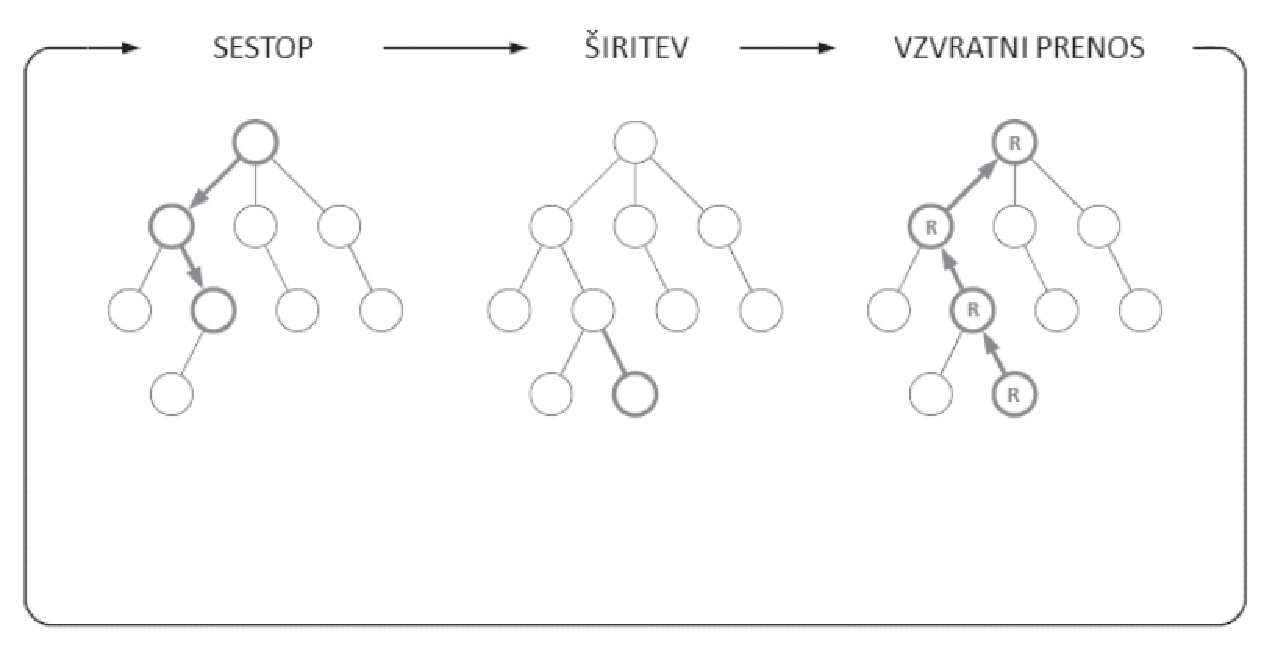
\includegraphics[width=0.8\textwidth]{photos/modifiedMCTS.pdf}
	\end{center}
	\caption{Na sliki je prikazano delovanje algoritma MCTS pri izvedbi algoritma AlphaZero, ki ga uporabljamo v diplomski nalogi. Ta MCTS ne uporablja postopka odigravanja stanj do konca igre, ampak izvede določeno število iteracij iskanja z raziskovalno funkcijo~\ref{iz:1}. }
	\label{modifiedMCTS}
\end{figure}

Uporaba algoritma MCTS je v tem algoritmu drugačna kakor v splošni uporabi.
Število iteracij je namenjeno biti veliko manjši, kakor v njegovi klasični uporabi, kjer je število iteracij več sto tisoč. 
MCTS pripomore k izboljšavi napovedi stanja, ki ga vrne nevronska mreža z raziskovanjem prostora.
Algoritem ne uporablja simulacij za pridobitev končnega stanja igre, napoved stanja, ki ga vrne nevronska mreža samo izboljša.

Vozlišče, ki ni bilo obiskano, se vzpostavi s napovedjo nevronske mreže in za tem vzvratno propagira napoved stanja.
Če je vozlišče končno stanje igre, vzvratno propagira končno stanje.
MCTS v tem primeru prejme par sto iteracij (v našem primeru 30 - 50) in ne več tisoč, kot jih izvajajo drugi algoritmi.
V sklopu diplomske naloge govorimo o MCTS iskanjih in ne odigravanjem, saj jih ta ne vpeljuje~\ref{modifiedMCTS}.


\begin{izrek}
	\label{iz:1}
	formula po kateri računa verjetnost zmage pri določeni akciji v algoritmu MCTS. Pričakovana vrednost akcije je določena z Q(s, a), ki predstavlja  pričakovano nagrado ob izbiri akcije v danem stanju igre, kateri je prišteta napoved nagrade P(s, a) ob izbiri akcije v danem stanju, ki ga vrne nevronska mreža, pomnoženo s raziskovalnim faktorjem in korenom števila vseh obiskov stanja igre v primerjavi s števili obiskov v danem vozlišču.
	\begin{equation}
	U(s, a) = Q(s, a) + c_{puct}P(s, a)\sqrt{\dfrac{\sum{N(s)}}{1+N(s, a)}}
	\label{eq:mctsFormula}
	\end{equation}
\end{izrek}

Glavno učenje algoritma poteka z igranjem iger, ki se za razliko od MCTS-ja odigrajo do konca in se dodajo v seznam učnih primerov.
Konec vsake iteracije igranja epizod iger se nevronska mreža uči na podlagi teh učnih primerov.
Za tem preveri moč novo naučenega modela z igranjem proti starejši različici modela in se shrani novi model samo če je boljši od starejšega za določen odstotek.
%%%%%%%%%%%%%%%%%%%%%%%%%%%%%%%%%%%%%%%%%%%%%%%%%%%%%%%%%%%%%%%%%%%%%%%%%%%%%%%%%%%%%%%%%%%%%%%%%%%%%%%%%%%%%%%%%%%%%%%%
%%%%%%%%%%%%%%%%%%%%%%%%%%%%%%%%%%%%%%%%%%%%%%%%%%%%%%%%%%%%%%%%%%%%%%%%%%%%%%%%%%%%%%%%%%%%%%%%%%%%%%%%%%%%%%%%%%%%%%%%
%%%%%%%%%%%%%%%%%%%%%%%%%%%%%%%%%%%%%%%%%%%%%%%%%%%%%%%%%%%%%%%%%%%%%%%%%%%%%%%%%%%%%%%%%%%%%%%%%%%%%%%%%%%%%%%%%%%%%%%%
%%%%%%%%%%%%%%%%%%%%%%%%%%%%%%%%%%%%%%%%%%%%%%%%%%%%%%%%%%%%%%%%%%%%%%%%%%%%%%%%%%%%%%%%%%%%%%%%%%%%%%%%%%%%%%%%%%%%%%%%
%%%%%%%%%%%%%%%%%%%%%%%%%%%%%%%%%%%%%%%%%%%%%%%%%%%%%%%%%%%%%%%%%%%%%%%%%%%%%%%%%%%%%%%%%%%%%%%%%%%%%%%%%%%%%%%%%%%%%%%%

\chapter{Opis pravil igre}
\label{chpravilaigre}

Igro smo opisali po Surag Nairjevi predlogi za igro AlphaZero, ki je na voljo na spletem gostovanju GitHub~\cite{alphazerogeneral}.
Strateško igro smo dodali kot modul, ki mora vsebovati definicijo igre in njena pravila, igralce, vizualizacijo in izgradnjo modela.
\textsl{}
Igra je določena s kvadratno mrežo 8 x 8, kjer polje lahko vsebuje največ eno figuro.
Ostale igre, ki so napisane za to različico AlphaZero izvedbe, kot na primer štiri v vrsto, gobang, othello, tri v vrsto, vsebujejo črno-bele figure.
Zakodirane so lahko z eno številko: -1 za igralca -1, +1 za igralca 1 ali 0, če je polje prazno.
Pri teh igrah je dimenzija kodiranja 2-dimenzionalna, kjer dimenzije predstavljajo višino in širino igralne plošče.
Pri RTS igrah moramo vedeti poleg igralca, komur ta figura pripada, tudi stanje te figure, na primer trenutno zdravje in njen tip.
Zato je prostor kodiranja 3-dimenzionalen, kjer je tretja dimenzija zakodirano stanje figure.
Če bi dovolili, da na posamezno polje spada več figur, se dimenzija ponovno poveča za 1.

Naš prvi poskus opisa igre je zelo spremenil Surag-Nairjevo implementacijo algoritma AlphaZero, saj smo stanja igre skozi algoritem prenašali nenumerično~\cite{objectAlphaZero}.
Hoteli smo ohraniti kompatibilnost z ovojnico algoritma, za katerega implementiramo svojo igro kot modul, kar je nenumerični zapis igre to preprečil.
Kompleksnejša implementacija igre je povzročila počasnejše igranje in učenje iger, saj je bilo preverjanje akcij počasnejše.

\section{Stanje igre}
\label{stanjeigre}
V tem razdelku bomo opisali zapis posamezne figure, njihove akcije in kaj naredijo in tip kodiranja stanja igre, ki ga potem sprejme nevronska mreža.

Igro smo opisali tako, da je čim bolj skladna s samim algoritmom AlphaZero, kot tudi da je njena aplikacija dovolj primerljiva z obstoječimi strateškimi igrami kot npr. StarCraft.
S tem v mislih, smo opisali nekaj preprostih pravil, ki jih ta igra upošteva:
\begin{itemize}
	\item figure se ne požirajo: vojaške figure ne napadejo drugih figur tako, da če je akcija napad možna, se postavijo na polje nasprotnikove figure in s tem prepišejo nasprotnikovikovo figuro in s tem jo uniči~\ref{picPoziranjeFigur}. 
	Vse figure imajo določeno zdravje, ki ga vojaške figure v večih korakih zmanjšajo z napadom,
	\item ena figura na polje: S tem ni možno blokiranje figur, s tem da se figura postavi na polje zlata in blokira nasprotnikovo figuro da jih nabere,
	\item igralec zgubi, če zgubi vse figure - več o ustavitvenih pogojih spodaj v razdelku~\ref{sKonecIgre},
	\item nabiranje zlatnikov je enkratna operacija, ki poteka podobno kot pri igri StarCraft, kjer mora figura pristopiti do polja zlata, zlatnike pobrati in jih za tem vrniti v glavno hišo.
	Nabiranje zlatnikov v tem primeru ne poteka tako, da se figura pomakne do polja zlata in s tem prične avtomatično pridobivati zlatnike, brez da bi jih vračal na odlagališče.

\end{itemize}

\begin{figure}[h]
	\begin{center}
		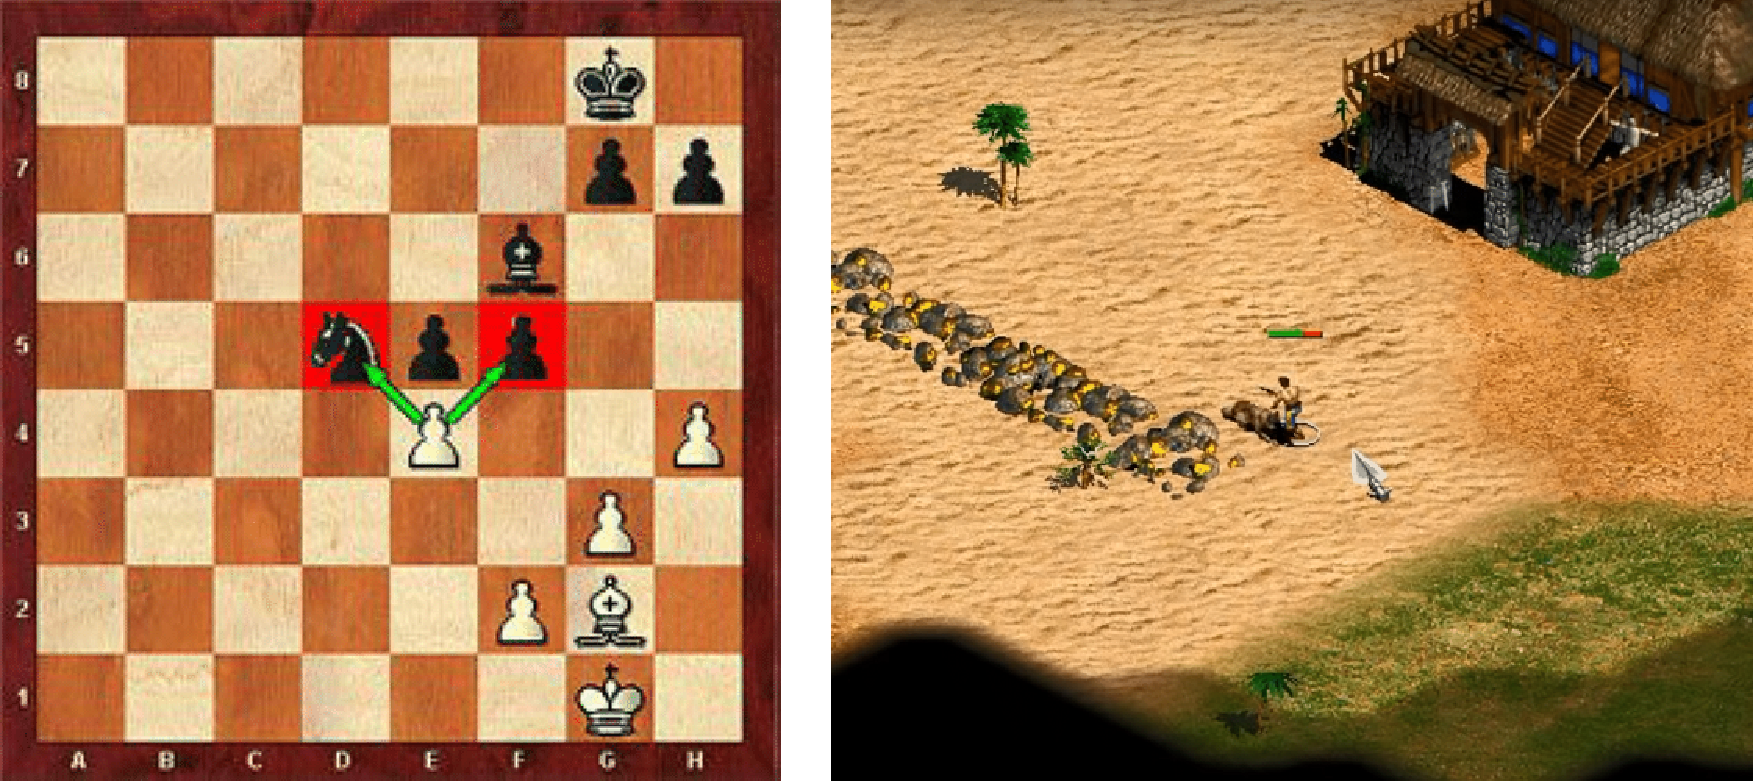
\includegraphics[width=1\textwidth]{photos/horizontal_health.pdf}
	\end{center}
	\caption{Na levi sliki je prikaz požiranja figur v igri šah, kjer se figura kmet lahko premakne na eno izmed dveh diagonalnih polj in s tem uniči trenutno nasprotnikovo figuro na tem polju. 
		Na desni sliki je prikaz vojskovanja delavca z volkom v igri Age of Empires II, kjer se figurama odšteva število življenjskih točk med napadanjem.}
	\label{picPoziranjeFigur}
\end{figure}

Sprva moramo opisati figure, ki bodo imele določeno vlogo v igri. Nabor figur je majhen, saj nočemo, da preiskovalni prostor postane prehitro prevelik.

\begin{table}
	\begin{center}
		\begin{tabular}{p{0.2\linewidth}|p{0.8\linewidth}}
			Ime figure        & {\tt Opis} \\ \hline
			{\tt polje zlata} & vir surovin, ki predstavljajo denar v igri, s katerim lahko igralec gradi nove stavbe in uri nove figure. 
								Vir zlata je neomejen in ne mora biti uničen \\
			{\tt delavec}     & figura namenjena gradnji stavb in nabiranju zlata \\
			{\tt vojašnica}   & stavba namenjena urjenju vojaških figur \\
			{\tt vojak}       & figura namenjena napadanju nasprotnikovih figur \\
			{\tt glavna hiša} & stavba namenjena urjenju delavcev in vračanju surovin zlata \\
		\end{tabular}
	\end{center}
	\caption{Določitev figur in njihovih namenov v igri. Definirali smo samo 5 figur, med katerimi je polje zlata nevtralna, saj je igralec ne more nadzorovati. }
	\label{tableFiguresDescription}
\end{table}

Na posameznem polju je lahko največ ena figura, tako da igralec ne more blokirati surovin zlata nasprotnemu igralcu, če to surovino ne obkoli v celoti.

Realizirali smo atribute figur. 
Pomembno je, da so te atributi numerični, da lahko podamo stanje igre kot N-dimenzionalen vektor, ki ga nevronska mreža lahko sprejme in se iz teh numeričnih podatkov uči.
Pomembno je, da ima vsako polje na šahovnici enako število atributov, tudi če je to polje prazno.
Vsako prazno polje ima vanj vpisan atribut čas igranja, ki je splošen za celo igro, vsa ostala polja imajo vrednost 0.


\begin{table}
	\begin{center}
		\begin{tabular}{p{0.2\linewidth}|p{0.8\linewidth}}
			Ime kodirnega polja    & {\tt Opis} \\ \hline
			{\tt ime igralca}      & določa igralca, h kateremu ta figura pripada. 
									 Igralec lahko nadzoruje samo svoje figure, izvaja akcije na svojih figurah in napada nasprotnikovikove figure \\
			{\tt tip figure}       & atribut predstavlja numerično predstavitev tifigure kot na primer polje zlata, delavec ipd.
									 Stanje igre potrebuje zapise tipov figur na poljih, da program ve, katere akcije tem figuram pripadajo\\
			{\tt trenutno zdravje} & koliko zdravja ima trenutna figura. 
									 Zdravje se lahko povečuje do nekega maksimuma z akcijo zdravi in znižuje z napadom figure \\
			{\tt nosi zlatnike}    & poseben atribut za delavce, ki predstavlja vrednost 1, če figura nosi zlatnike in 0, če ga ne nosi. 
									 To se upošteva pri nabiranju in vračanju zlata, kjer se ti dve akcije ne zgodita v roku ene poteze, ampak se mora stanje prenašati skozi več potez \\
			{\tt denar}            & trenutna količina zbranega denarja za posameznega igralca. 
									 To polje se ob spremembi količine denarja spremeni v vseh figurah tega igralca \\
			{\tt čas igranja}      & to polje predstavlja koliko potez se je v trenutni igri že izvedlo. 
									 Atribut je prisoten v vseh poljih in se spremeni v vseh poljih šahovnice, ko se izvede nova akcija \\
		\end{tabular}
	\end{center}
	\caption{Definicija on opis kodirnikov stanja igre, s katerimi je predstavljeno vsako polje na šahovnici. Več o kodiranju teh polj si bomo pogledali v sekciji kodiranja~\ref{kodiranja}.}
	\label{tableEncoders}
\end{table}

Poseben primer je figura polje zlata, ki ne pripada nobenemu igralcu v večini RTS igrah. 
V tem primeru smo podali vsakemu igralcu svoje polje zlata, da je igra simetrična in nevronska mreža ne interpretira prazno polje igralca kot prazno polje.
Figuri polje zlata se ne spreminja atribut zdravja, saj jo ne moremo poškodovati. 
Zlata je neomejeno in ko igralec odloži zlatnike v glavno hišo, se vsem figuram tega igralca nastavijo zlatniki na novo dobljeno vrednost. 
Pri izgradnji nove stavbe ali urjenju figure število zlatnikov zmanjša za vse figure tega igralca.

\section{Akcije}

\begin{figure}[h]
	\begin{center}
		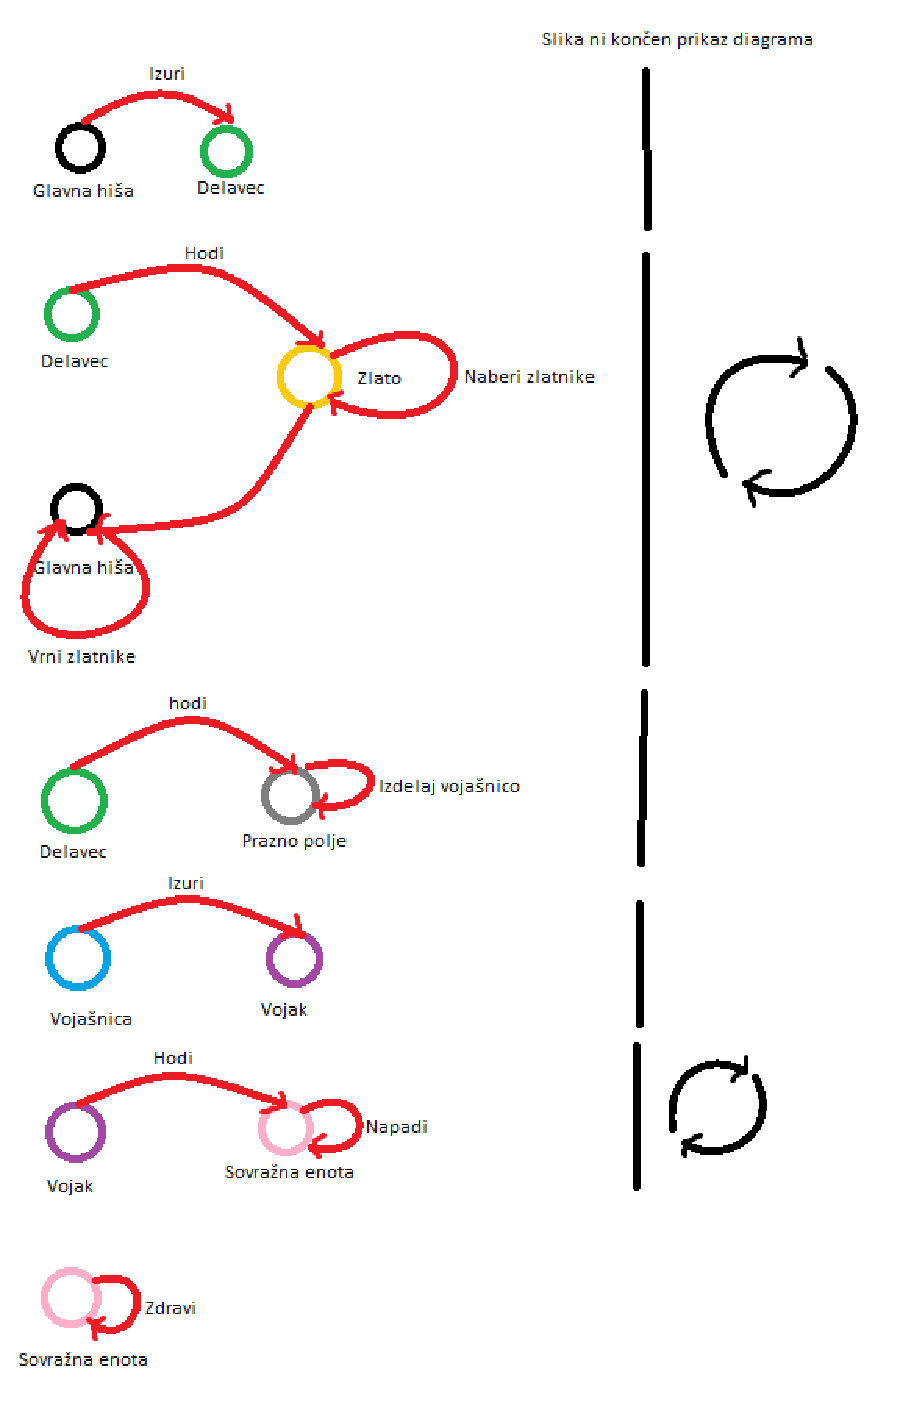
\includegraphics[width=1\textwidth]{photos/prikazAkcij.pdf}
	\end{center}
	\caption{Slika prikazuje diagram poteka možnih akcij in njihovih rezultatov ob določenih pogojih.}
	\label{picActions}
\end{figure}

Pri opisu pravil igre smo tudi določili akcije~\ref{picActions}, ki jih igralčeve figure lahko izvajajo. 
Vsaka figura ne more izvajati vseh akcij, kot na primer stavbe se ne morejo premikati, same figure kot delavec in vojak ne morejo uriti novih figur~\ref{tabelfigures}.

\begin{table}
	\begin{center}
		\begin{tabular}{p{0.3\linewidth}|p{0.7\linewidth}}
			Ime akcije                          & {\tt Opis} \\ \hline
			{\tt premiki (4 smeri)}             & figuri vojak in delavec se lahko premakneta na sosednje polje na šahovnici, če je to mesto prazno \\
			{\tt naberi zlatnike}               & delavec lahko nabere zlatnike če je v neposredni bližini figure polje zlata. Zlatnike za tem drži pri sebi, pri katerem se nastavi zastavica nosi zlatnike\\
			{\tt vrni zlatnike}                 & delavec vrne zlatnike, ki jih drži pri sebi v glavno hišo, na kar se igralcu prišteje denar \\
			{\tt napadi (4 smeri)}              & vojak lahko napade nasprotnikovo figuro, če je ta v neposredni bližini in jo rani za določen faktor. Če figuri ne preostane več življenjskih točk je eliminirana s šahovnice, kot je tudi igralec, če je bila eliminirana njegova zadnja figura \\
			{\tt izuri delavca (4 smeri)}       & glavna hiša lahko izuri novo figuro delavec, če ima dovolj denarja, na kar se igralcu odšteje denar\\
			{\tt izuri vojaka (4 smeri)}        & vojašnica lahko izuri novo figuro vojak, če ima dovolj denarja, na kar se igralcu odšteje denar \\
			{\tt izgradi vojašnico (4 smeri)}   & delavec lahko izgradi vojašnico na prazno mesto zraven njega, na kar se igralcu odšteje denar \\
			{\tt izgradi glavno hišo (4 smeri)} & delavec lahko izgradi glavno hišo na prazno mesto zraven njega, na kar se igralcu odšteje denar \\
			{\tt zdravi (4 smeri)}              & figura lahko zdravi sosednjo prijateljsko figuro, če ta nima polnega življenja, na kar se igralcu odšteje denar\\
		\end{tabular}
	\end{center}
	\caption{Opis akcij, njihovih dejanj in pogojev, ki morajo biti izpolnjeni, da se akcija lahko izvrši. Nekatere akcije imajo 4 smeri izvajanja, kar pomeni, da bo akcija npr. izuri delavca dol povzročila, da se izuri delavec na južni strani glavne hiše.}
	\label{tableActions}
\end{table}

Sprva smo določili nekatere izmed zgornjih akcij, na način izbire prvega mesta med sosednjimi polji, ki ustreza akciji. 
Naslednje akcije so se izvajale po zaporedju~\ref{pickorakiPreverjanja}:
\begin{itemize}
	\item naberi zlatnike,
	\item vrni zlatnike,
	\item napadi,
	\item delavec,
	\item vojak, 
	\item vojašnica,
	\item glavna hiša,
	\item zdravi.
\end{itemize}
\begin{verbatim}
koordinate = [(x - 1, y + 1),
              (x, y + 1),
              (x + 1, y + 1),
              (x - 1, y),
              (x + 1, y),
              (x - 1, y - 1),
              (x, y - 1),
              (x + 1, y - 1)]
for sosednji_x, sosednji_y in koordinate:
    # preveri pogoj akcije
    if (pogoj == ok):
        return sosednji_x, sosednji_y
\end{verbatim}

\begin{figure}[h]
	\begin{center}
		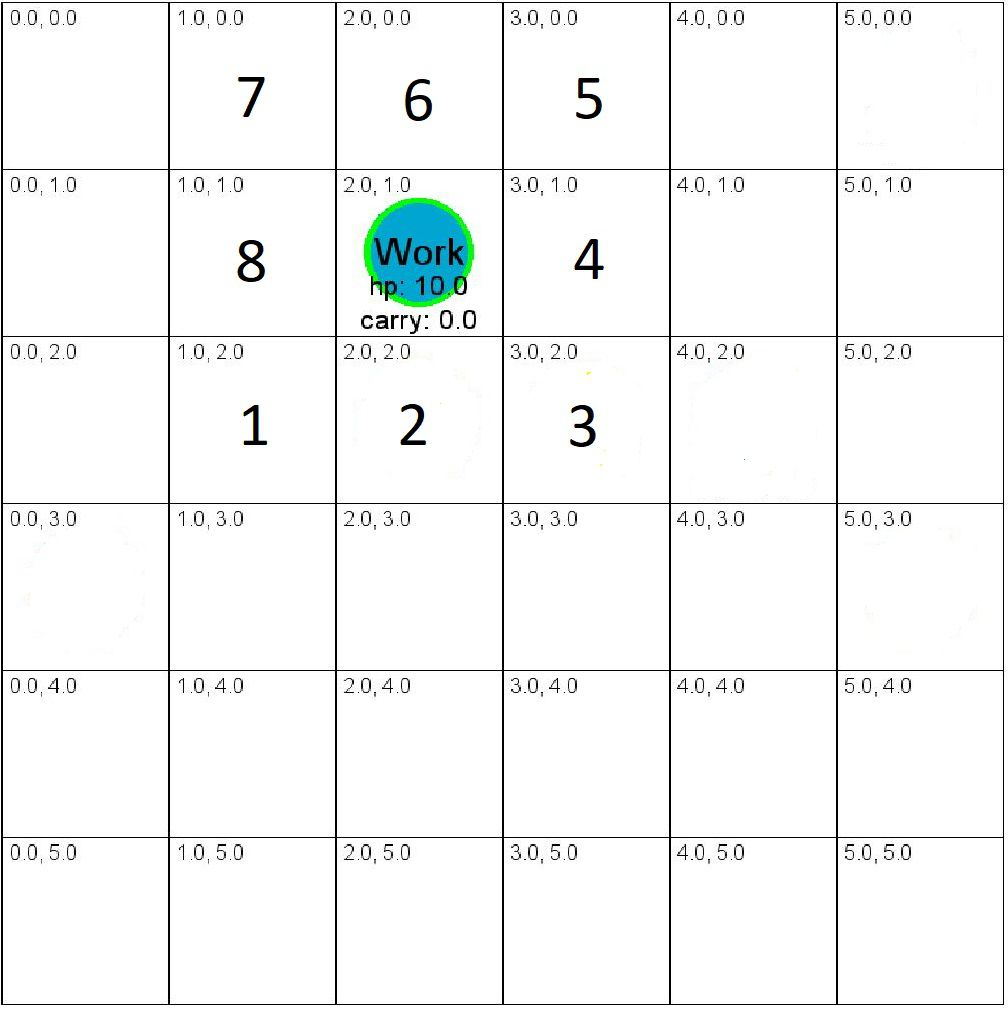
\includegraphics[width=0.6\textwidth]{photos/korakiPreverjanja.pdf}
	\end{center}
	\caption{Na sliki je s številkami označeno zaporedje, v katerem se izvedejo zgoraj navedene akcije. Sprva se vzpostavijo sosednje koordinate, za tem se po zaporedju od prve do zadnje koordinate preverja veljavnost polj. Ko je doseženo prvo veljavno polje, se izbere to polje kot primerno. }
	\label{pickorakiPreverjanja}
\end{figure}



Ko je doseženo prvo prazno polje v tem zaporedju, se tam izgradi nova stavba ali izuri nova figura.
Ko je prva nasprotnikova figura izbrana v tem zaporedju, je napadena.
Rezultat tega je gradnja stavb in urjenja figur v spodnji levi kot šahovnice, saj so izbrana prva polja v zaporedju, kot na primer x-1, y+1, in širjenje proti zgornjim desnim kotom, ko so vsa ostala polja zasedena, oziroma tam ni nasprotnikovih figur.

Algoritem smo popravili tako, da smo spremenili te akcije (razen naberi zlatnike in vrni zlatnike), da so posamezne akcije za vsako izmed štirih sosednjih polj.
Za vpeljavo posameznih akcij smo se odločili, ker ne moramo izbrati polja po zgornjem zaporedju tako, da bi bilo za oba igralca enako.

\section{Kodiranja}
\label{kodiranja}
\begin{table}

	\begin{center}
		
	\begin{tabular}{p{0.2\linewidth}|p{0.4\linewidth}|p{0.1\linewidth}|p{0.1\linewidth}}
		Ime figure          & {\tt Akcije}                                                              & {\tt Zdravje} & {\tt Strošek izdelave} \\ \hline
		{\tt polje zlata}   & /                                                                         & 10            & 0 \\
		{\tt delavec}       & smeri premikanja, vojašnica, glavna hiša, naberi in vrni zlatnike, zdravi & 10            & 1 \\
		{\tt vojašnica}     & vojak, zdravi                                                             & 10            & 4 \\
		{\tt vojak}         & smeri premikanja, napad, zdravi                                           & 20            & 2 \\
		{\tt glavna hiša}   & delavec, zdravi                                                           & 30            & 7 \\
	\end{tabular}
	\end{center}
	\caption{Tu so opisane figure z njihovimi akcijami in nastavljenimi atributi.}
	\label{tabelfigures}
\end{table}

Določili smo začetno stanje vsake igre, kjer sta igralca postavljena v sredino mreže z njihovima glavnima hišama, zraven njiju ima vsak igralec svoje polje zlata. 
Vsakemu igralcu se doda na začetku določena količina denarja za izgradnjo začetnih delavcev. V našem primeru je bilo to 1, tako da je lahko izgradil samo enega delavca.

Sedaj smo potrebovali zakodirati to stanje igre, v numerični prikaz, ki ga bo nevronska mreža lahko interpretirala. 
To stanje lahko zakodiramo z desetiškim kodiranjem, vendar obstaja možnost, da nevronska mreža sloni proti boljšim obravnavanjem pozitivnih števil za igralca +1, kot za igralca -1. 
Ravno iz tega razloga obstaja kodiranje z enico v zapisu vsakega stanja (ang. one-hot encoding), ki spremeni desetiška števila v binarni vektor~\ref{oneHotEncoder}.

Akciji naberi in vrni zlatnike, ostaneta vedno po 1 akcijo, ker za delavca ni razlika, iz katerega sosednjega polja zlata vzame zlatnike, kot ni razlike pri vračanju njih.

\subsection{Desetiško}
Pri desetiškim kodiranjem, predstavimo vsak atribut figure z eno desetiško številko.
Ker imamo figure s 6 atributi, lahko stanje zakodirane igre predstavimo z dimenzijami širina x višina x 6.

Igralec predstavlja številko -1 za igralca -1, 1 za igralca 1 in 0 za prazno polje.
\subsection{Kodiranje z enicami v zapisu}
\label{oneHotEncoder}
\begin{table}
	\begin{center}
		\begin{tabular}{p{0.2\linewidth}|p{0.2\linewidth}|p{0.6\linewidth}}
			Ime kodirnega polja      & {\tt št kodirnih bitov} & {\tt Opis} \\ \hline
			{\tt ime igralca}        & 2                       & figura na polju je lahko predstavljena s 2 biti zaradi treh različnih možnosti: 00 predstavlja prazno polje, 01 predstavlja igralca 1 in 10 igralca -1 \\
			{\tt tip figure}         & 3                       & predstaviti moramo 5 različnih figur, kar lahko zakodiramo z najmanj 3 biti\\
			{\tt trenutno zdravje}   & 5                       & nekatere figure imajo veliko življenjskih točk (npr. glavna hiša 30), za kar moramo uporabiti 5 bitov. 
																 Uporabili smo večje število življenjskih točk, tako da lahko uspešno deluje ranjujoča funkcija~\ref{destroy_formula_2018_11_17}, da figure ne eliminira prehitro \\
			{\tt nosi zlatnike}      & 1                       & zastavica ki se postavi na 1, ko figura delavec nosi zlatnike, drugače je postavljena na 0 \\
			{\tt denar}              & 5                       & za ta kodirnik smo uporabili večje število, saj pustimo da igralec gradi ekonomijo in shranjuje denar, da ga potem lahko na hitro zapravi na figurah, ko ga ima dovolj za njihovo izgradnjo.
																 To lahko privede v zanimive taktike hranjenja denarja in za tem hitro izgradnjo vojaških enot za napad nasprotnikovih figur \\
			{\tt čas igranja}        & 11                      & $2^{11}$ = 2048, kar pusti igralcu dovolj časa da odkriva nove poteze, ampak ga dovolj hitro omeji, da se konča igra in začne nova \\
		\end{tabular}
	\end{center}
	\caption{Predstavitev število kodirnih atributov za posamezni kodirnik in pojasnitev odločitve za število kodirnih bitov. }
	\label{tableEncodersOneHot}
\end{table}

Dimenzija zakodiranega prostora je tako 8 x 8 x 22, kar je 3.6-krat števil, ki kodira posamezno stanje igre.
To zna otežiti učenje nevronske mreže, ker ima s tem kodiranjem več števil, pri katerih mora ugotoviti primernost posameznega števila.

\section{Konec igre}
\label{sKonecIgre}
Konec igre se izvede pod določenimi pogoji:
\begin{itemize}
	\item igralec nima za izvesti več nobene možne akcije,
	\item vse figure igralca so uničene,
	\item ko se izteče čas.
\end{itemize}

Določiti smo morali umeten konec igre, zaradi primera, kjer se igra nikoli ne zaključi, da se na primer delavci premikajo v ciklu in se tako igra nikoli ne konča.
S tem smo povišali prednost aktivnim igralcem, ki nabirajo zlatnike in imajo več enot kakor nasprotni igralec.

\subsection{Reševanje problema neskončnega števila potez}
\label{sKillFunction}
Čakanje, da se čas igre izteče, je problematično, saj učenje modela poteka zelo počasi, posebej ko MCTS raziskuje prostor.
Za to smo razvili funkcijo, ki prisili model k izvajanju akcij v zgodnem času igre, drugače se figuram preveč začnejo zmanjševati življenjske točne in so zato eliminirane s šahovnice.


\begin{figure}[h]
	\begin{center}
		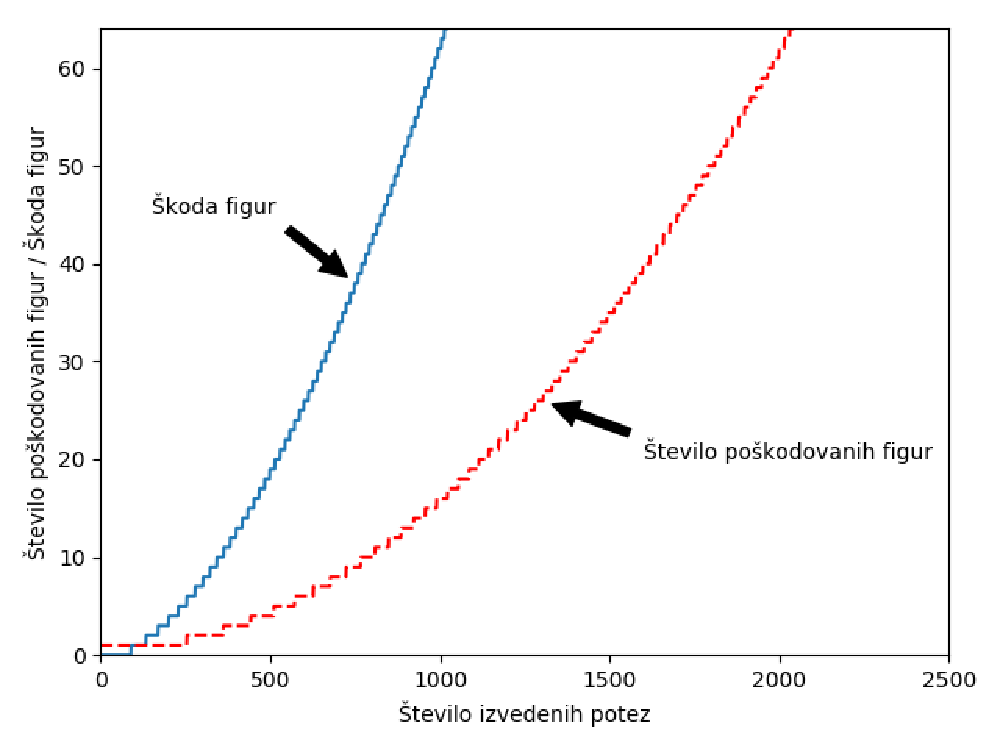
\includegraphics[width=0.8\textwidth]{photos/destroy_formula_2018_11_17.pdf}
	\end{center}
	\caption{Na grafu sta narisani dve funkciji, ki določata zmanjšanje življenjskih točk se obravnava v določeni figuri v danem času igre(modra) in koliko igralcev je bilo poškodovanih v trenutnem časovnem okviru(rdeča).}
	\label{destroy_formula_2018_11_17}
\end{figure}


Vidimo, da je krivulja zmanjšanja življenjskih točk veliko bolj stroga in se v igri začenja že zelo zgodaj. 
To je zato, ker želimo hitro odpraviti nedejavnih igralcev in  tiste, ki zbirajo zlatnike in pridobivajo nove figure.
Vidimo tudi y osi od 0 do 64, kar je največje število igralcev za enega igralca, tako da bo pri približno 2000 korakih vsaka figura dobil smrtno poškodbo, zato časovni potek nikoli ni dosežen.

Figure lahko tudi uporabijo akcijo zdravljenja, s čimer povečajo trenutno zdravje določene figure do največ njenega maksimuma.
	
Z zgoraj določeno funkcijo je bil problem določiti pravšnjo stopnjo količine zmanjšanja življenjskih točk figur in izločevanje neaktivnih igralcev dovolj zgodaj v igri, in sicer problem z balansiranjem količine in stroškom zdravljenja. 
Če so bili stroški dovolj nizki, so igralci stalno samo zdravili figure in končali igro pri približno tisoč potezah, kar je pregloboko za normalno igro.
Za to je bilo potrebno povišati strošek zdravljenja, kar je privedlo do hitrejšega nenadnega umiranja figur, saj igralci niso imeli dovolj kovancev za zdravljenje, na kar je bilo potrebno povišati količino vrnjenih kovancev iz figure zlato.

\subsection{Ustavitveni pogoj}
Ustavitveni pogoj deluje tako, da se na številu določenih potez igra preprosto prekini in oceni zmagovalca po eni izmed spodaj navedenih formul.
Igra se prekine po 100 - 200 potezah, če si do takrat igralca med sabo nista uničila figur.
V spodnjih treh  enačbah sta označena igralec 1 z oznako p1 in igralec 2 z oznako p2.

\begin{izrek}
	\label{ustavitvenipogoj1}
Prvi: igralec 1 zmaga, če ima več denarja kot igralec 2
	\begin{equation}
p1.zlatniki > p2.zlatniki
	\label{eq:ustavitvenipogoj1}
	\end{equation}
\end{izrek}

Prvi izrek je dober ustavitveni pogoj, za testiranje igralcev pri nabiranju zlatnikov, kjer zmaga preprosto tisti, ki jih nabere več.

\begin{izrek}
	\label{ustavitvenipogoj2}
Drugi: igralec 1 zmaga, ko je seštevek zdravja vseh figur igralca 1 je večji od seštevka zdravja vseh figur igralca 2
	\begin{equation}
	\sum{p1.figure.zdravje} > \sum{p2.figure.zdravje}
	\label{eq:ustavitvenipogoj2}
	\end{equation}
\end{izrek}

Če je pogoj za zmago večje število življenja svojih figur kakor nasprotnikovih hkrati pomeni, da lahko igralec nabira več zlatnikov in z njimi gradi nove stavbe in uri nove enote, kar zagotavlja za igralca večjo skupno vsoto življenja figur in hkrati zagotavlja težo k urjenju vojaških enot z namenom, da nasprotnikovim enotam zmanjša število življenjskih točk.

\begin{izrek}
	\label{ustavitvenipogoj3}
Tretji: igralec 1 zmaga, ko je seštevek zdravja vseh figur igralca 1 plus njegov denar je večji od seštevka zdravja vseh figur igralca 2 plus njegov denar
	\begin{equation}
	\sum{p1.figure.zdravje} + p1.zlatniki > \sum{p2.figure.zdravje} + p2.zlatniki
	\label{eq:ustavitvenipogoj3}
	\end{equation}
\end{izrek}

K drugemu izreku smo pripeli trenutno število shranjenih zlatnikov igralca, kar dodatno doprinaša motivacijo igralca k nabiranju novih zlatnikov.
V večini učnih primerov, kot smo to opisali v poglavju rezultati~\ref{chrezultati}, smo uporabljali tretji ustavitveni pogoj~\ref{ustavitvenipogoj3}, saj združuje tako življenjske točke enot, kot tudi denarja.
Vendar imajo figure običajno veliko več življenjskih točk kolikor so vredne denarja, tako da je izgradnja nove figure za igralca primernejša, kot da bi denar shranjeval.

%%%%%%%%%%%%%%%%%%%%%%%%%%%%%%%%%%%%%%%%%%%%%%%%%%%%%%%%%%%%%%%%%%%%%%%%%%%%%%%%%%%%%%%%%%%%%%%%%%%%%%%%%%%%%%%%%%%%%%%%
%%%%%%%%%%%%%%%%%%%%%%%%%%%%%%%%%%%%%%%%%%%%%%%%%%%%%%%%%%%%%%%%%%%%%%%%%%%%%%%%%%%%%%%%%%%%%%%%%%%%%%%%%%%%%%%%%%%%%%%%
%%%%%%%%%%%%%%%%%%%%%%%%%%%%%%%%%%%%%%%%%%%%%%%%%%%%%%%%%%%%%%%%%%%%%%%%%%%%%%%%%%%%%%%%%%%%%%%%%%%%%%%%%%%%%%%%%%%%%%%%
%%%%%%%%%%%%%%%%%%%%%%%%%%%%%%%%%%%%%%%%%%%%%%%%%%%%%%%%%%%%%%%%%%%%%%%%%%%%%%%%%%%%%%%%%%%%%%%%%%%%%%%%%%%%%%%%%%%%%%%%
%%%%%%%%%%%%%%%%%%%%%%%%%%%%%%%%%%%%%%%%%%%%%%%%%%%%%%%%%%%%%%%%%%%%%%%%%%%%%%%%%%%%%%%%%%%%%%%%%%%%%%%%%%%%%%%%%%%%%%%%

\chapter{Učenje modela}
\label{chucenjemodela}
Ena izmed glavnih komponent učnega postopka je seveda nevronska mreža, ki hrani moči povezav določenih akcij ob določenem stanju igre.
V tem poglavju bomo sprva predstavili zgradbo nevronske mreže iz tehničnega vidika, nato se bomo posvetili prestavitvi parametrov, ki so nastavljivi pri postopku učenja in od njih je odvisno, koliko časa in na kakšen način se bo naš model učil ob nastavljeni konfiguraciji igre.
Proti koncu poglavja se bomo poglobili v možno tehniko postopnega učenja modela, kjer inkrementalno dodajamo zahtevnejše konfiguracije in pravila igre.

\section{Zgradba nevronske mreže}

V sklopu te diplomske naloge se nismo podajali v spreminjanje zgradbe nevronske mreže, temveč smo vzeli že izgrajeno nevronsko mrežo, primerno za učenje igre Othello.
To ni najprimernejši pristop, kar je mogoče tudi poslabšal zmožnost in hitrost učenja modela, o čemer smo več prediskutirali v poglavju~\ref{chdiskusija}.

Uporabili smo modul Keras znotraj TensorFlow knjižnice, za implementacijo modela nevronske mreže.
Programska koda za izgradnjo modela je lažje berljiva v modulu Keras kakor v TensorFlow, zato smo se zanj tudi odločili.
Ker je Keras impementiran znotraj TensorFlow knjižnice od verzije 1.9 izdani leta 2017, ni bilo večjih težav z inštalacijo te knjižnice na odjemalčevem računalniku z vtičnikomm tensorflow-ue4.

Model za vhod vzame učne množice stanja iger dimenzij širina x višina x število kodirnikov, kar je v našem primeru 8 x 8 x 6.
Potem gre ta učna množica skozi 4 konvolucijske nivoje, kjer je velikost filtra 3.
Prva dva konvolicijska nivoja imata oblogo ničel okrog matrike, tako da se velikost konvolucijskega nivoja ne zmanjša, druga dva tega obloge nimata, kar zniža velikost nivoja iz 8 na 4.
tako da je izhod zadnjega konvolucijskega nivoja dimenzije velikost serije  x (širina - 4) x (višina - 4) x število kanalov
Vsak izhod konvolucijskih nivojev se s postopkom normalizacijo serije (ang. batch normalization) normalizira aktivacijo prejšnjega nivoja ob vsaki seriji, izhodi tega se preuredijo z relu aktivacijsko funkcijo, ki za vsa negativna števila vzame vrednost 0.
Za tem se izhod zadnjega nivoja normalizirane konvolucije izravna v 1-dimenzionalni vektor in se poda dvema polno povezanima nivojema, ki sta ponovno normalizirana z normalizacijo serije.
Tedva nivoja sta potem ponovno spuščena skozi aktivacijsko funkcijo relu podana v  Dropout funkcijo, ki prepreči prekomerno prileganje.

Za tem je izgrajen polno povezan nivo Pi, ki ima toliko število izhodov, koliko je možno število akcij v igri za vsako celico, ki ima aktivacijsko funkcijo softmax,
Izgrajen je tudi polno povezan nivo V, ki ima en izhod, ki predstavlja zmago ali poraz z tanh aktivacijsko funkcijo.
Za izhod Pi se nastavi funkcija izgube kategorična prečna entropija, za izhod V  srednja napaka korena (mean-squared error).

\begin{figure}[h]
	\begin{center}
		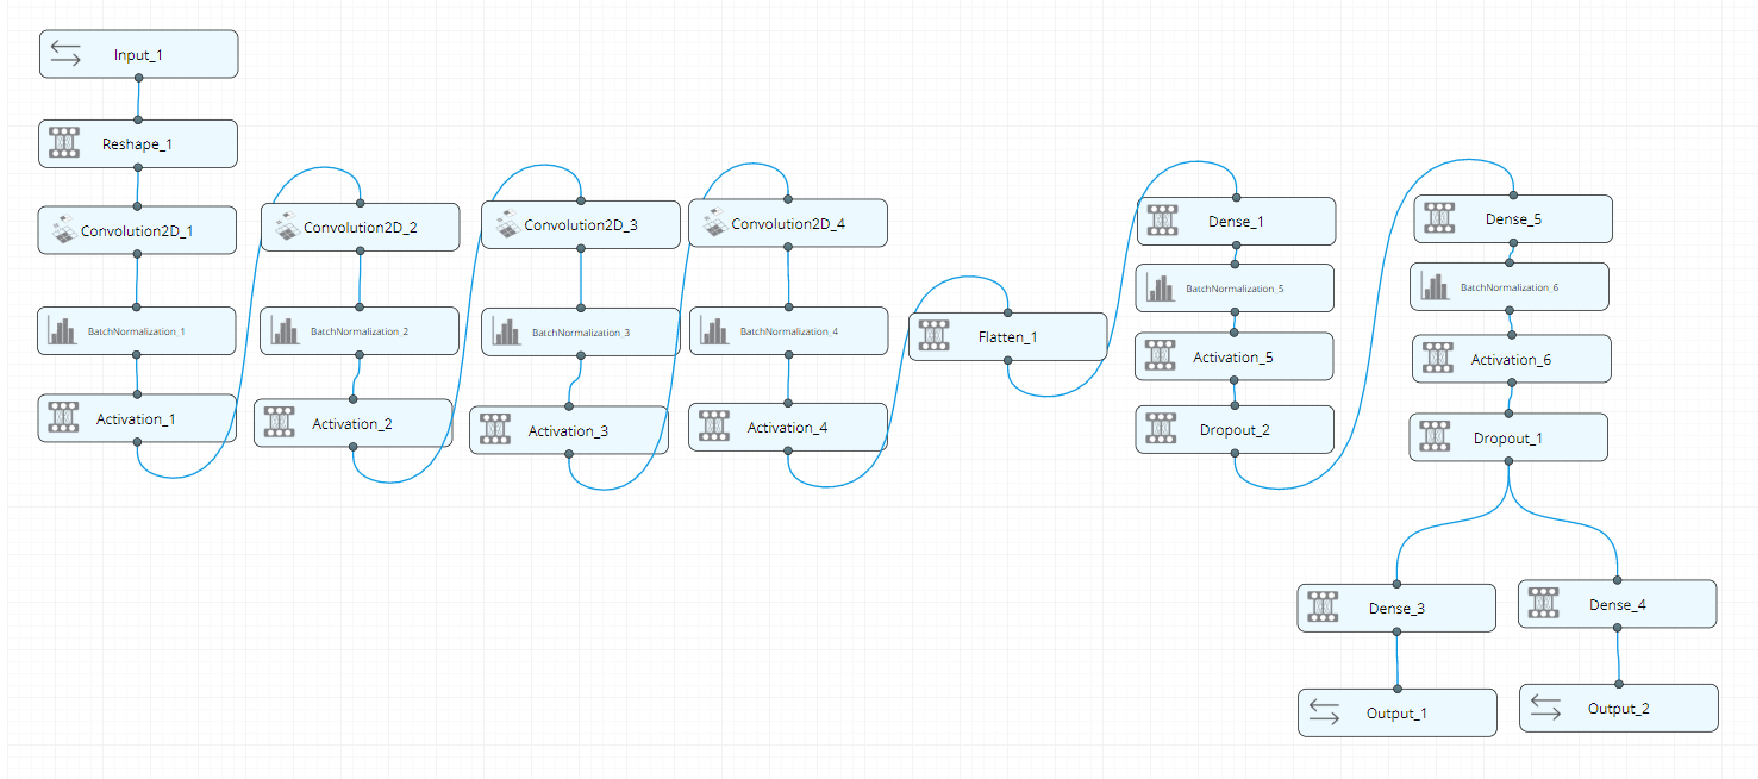
\includegraphics[width=1\textwidth]{photos/model_using_deepcognition.pdf}
	\end{center}
	\caption{Model nevronske mreže, uporabljen za učenje igre. Izgrajen je iz štirih konvolucijskih nivojev, med katerimi je izhod normaliziran in spuščen skozi relu aktivacijsko funkcijo. Nato se poda izhod zadnjega konvolucijskega nivoja v dva polno povezana nivoja, za katerima se določi izhod V in Pi, ki predstavljata napoved zmage (V) in napovedi verjetnosti akcij (Pi).
		Slika je bila izdelana z uporabo aplikacije Deep Learning Studio~\cite{deepcognition}.}
	\label{vizualzacijaModela}
\end{figure}



\section{Predstavitev parametrov}
\label{parametri}
Učni algoritem uporablja množico parametrov za učenje.
Ti predstavljajo različno število iteracij igranja iger (iteracije in epizode igranja), kot tudi iteracij učenja nevronske mreže (epohi).
Predstavljajo tudi same nastavitve raziskovanja algoritma MCTS (C\textsubscript{puct}) in število primerjav, kateri naučen model je boljši.

V tabeli opisa parametrov~\ref{tableParameters1} so predstavljeni najpomembnejši parametri, ki smo jih spreminjali ob učenju modela na naši RTS igri.

\begin{table}
	\begin{center}
		\begin{tabular}{p{0.15\linewidth}|p{0.15\linewidth}|p{0.7\linewidth}}
			Ime parametra                             & {\tt Privzeta vrednost} & {\tt Opis} \\ \hline
			{\tt C\textsubscript{puct}}               & 1 						& parameter drevesnega raziskovanja, ki vpliva direktno na raziskovanje MCTS algoritma. 
																				  Večja kot je vrednost parametra, bolj bo MCTS dajal prednost neraziskanim vozlišči. V našem primeru smo izbrali vrednost 1 in s tem nismo prispevali k dodatni uteži k raziskovanju.\\
			{\tt število iteracij}                    & 30 - 60					& predstavlja število učenj algoritma na odigranih igrah in število izbire boljšega modela.
																				  Parameter tudi predstavlja, kolikokrat se bo igra odigrala v celoti, kjer bo konec predstavljal končni pogoj oziroma eliminacija nasprotnika.\\
			{\tt število epizod}                      & 8 						& nam zagotovi pridobitev dovolj velikega nabora odigranih iger, nad katerimi se potem algoritem uči.
																				  Vsako epizodo se odigra število iger, kolikor je nastavljeno s parametrom število iteracij.\\
			{\tt število MCTS iskanj}                 & 30 - 50					& predstavlja število raziskanih vozlišč v iteraciji igre. 
														 						  MCTS iskanja se ne izvršijo do konca igre, ampak do neraziskanega vozlišča oziroma če je raziskano vozlišče konec igre.
														 						  Bodimo pozorni na majhno število MCTS iskanj (30 - 50), za razliko od tradicionalnih MCTS algoritmov, ki na primer v igri šah odigrajo več 10-tisoč iteracij~\cite{kohne}.\\
		
		\end{tabular}
	\end{center}
	\caption{Tabela 1/2 o opisu parametrov.}
	\label{tableParameters1}
\end{table}

\begin{table}
	\begin{center}
		\begin{tabular}{p{0.15\linewidth}|p{0.15\linewidth}|p{0.7\linewidth}}
			Ime parametra                             & {\tt Privzeta vrednost} & {\tt Opis} \\ \hline

			{\tt število primerjanj modelov}  		  & 10 						& kolikokrat se bosta trenutni model k se uči in njegova prejšna različica pomerila med sabo, da se ohrani boljši.
																				  Naučena modela se med sabo pomerita z igranjem iger od začetka do konca, kjer je rezultat zmaga nekoga izmed modelov, oziroma neodločeno.\\
			{\tt število iteracij učnih primerov}     & 8 						& nam zagotavlja, da ohranjamo novejše učne primere in starejše zavržemo.
																				  Vsako epizodo se doda nova zbirka iger ter odstrani najstarejša, če število shranjenih epizod presega ta parameter.
																				  To nam zagotavlja dovolj svežo učno množico, nad katero se nevronska mreža uči.
																				  V našem primeru je bil nastavljen na manjšo vrednost (8), saj kodiranja stanj naše igre zasedejo veliko pomnilnika.\\
			{\tt epohi}     						  & 100 					& Število iteracij učenja nevronske mreže skozi učne primere.\\
		\end{tabular}
	\end{center}
	\caption{Tabela 2/2 o opisu najpomembnejših učnih parametrov, uporabljenih pri učenju algoritma AlphaZero. Pri parametrih so zapisane tudi njihove okvirne oziroma največkrat uporabljene konfiguracijska števila.}
	\label{tableParameters2}
\end{table}



\section{Postopno učenje}
Učenje te igre je zapleteno zaradi pogojev konca igre. 
Algoritem izvaja igranje igre dokler ne doleti do ustavitvenega pogoja, ta pri RTS igri lahko ni nikoli dosežen, saj se lahko vojaška enota stalno premika v istem krogu, kakor bi se lahko trdnjava vedno premikala samo po dveh istih poljih.
Cikel akcij se lahko reši z uporabo časovnih omejitev, kjer se igranje igre ustavi ko se izteče čas, vendar to povzroča površnejši približek ocene stanja igre, ki vpliva na učenje nevronske mreže.
Zaradi kompleksnejšega ustavitvenega pogoja lahko model hitro prekomerno prilagodi na napačno igranje igre.
Dober primer je ustavitveni pogoj z vsoto zdravja igralčevih enot in njegovih trenutnih zlatnikov~\ref{eq:ustavitvenipogoj3}, kjer se igralca ne naučita pravilno napadati nasprotnikovih enot, da znižujeta nasprotnikove življenjske točke, ampak konstantno nabirata nove zlatnike in gradita in urita nove enote.
Ker igralca nista naučena zaključiti igro z eliminacijo nasprotnikovih enot.

Iz tega razloga, se nam je porodila učna ideja s postopnim učenjem modela. 
Ideja govori o spreminjanju pravil iger in nastavitev parametrov med učenjem.
S tem bi lahko v začetnih fazah učenja dali prednost nabiranju zlatnikov in s tem naučil algoritem uspešnega in hitrega nabiranja, kot na primer ustavitveni pogoj 1~\ref{eq:ustavitvenipogoj1}.
Za tem bi ta naučeni model nagradil na tak način, da bi mu spremenil ustavitveni pogoj na 2~\ref{eq:ustavitvenipogoj2} in h konfiguraciji akcij dodal možnost gradnje stavb, s čimer bi zdajšnji model, ki dobro nabira zlatnike z nadaljnjim učenjem nadgradil da poleg nabiranja gradi hiše in s tem povečuje število življenjskih točk enot, ki jih igralec obvladuje.
Ta model bi v tretji fazi nadgradil z akcijami urjenja vojaških enot in napadom drugega igralca.

Poskusili smo naučiti model po zgoraj opisanem postopku, vendar učenje ni potekalo uspešno.
Nevronska mreža je vzpostavila začetna stanja vrednosti vozlišč akcij po vnaprej naučenih utežeh pridobljenih iz naučenega modela, ki v fazi 2 ali 3 ni vseboval novo dodanih akcij kot gradnja stavb oziroma napadanje.
Zaradi majhnega ocenjenega stanja novih akcij, so te manjkrat obiskane in zato manj raziskane.
Algoritem zaradi sprememb pravil igre deluje zelo naključno, saj naučene uteži delujejo v nasprotju igralčevih želja.
MCTS pri tem iskanju ne pripomore veliko, saj so neraziskana stanja igre vzpostavljena glede na uteži iz nevronske mreže, stanje  se popravi ko doseže končno stanje, kar se zgodi redko.

%%%%%%%%%%%%%%%%%%%%%%%%%%%%%%%%%%%%%%%%%%%%%%%%%%%%%%%%%%%%%%%%%%%%%%%%%%%%%%%%%%%%%%%%%%%%%%%%%%%%%%%%%%%%%%%%%%%%%%%%
%%%%%%%%%%%%%%%%%%%%%%%%%%%%%%%%%%%%%%%%%%%%%%%%%%%%%%%%%%%%%%%%%%%%%%%%%%%%%%%%%%%%%%%%%%%%%%%%%%%%%%%%%%%%%%%%%%%%%%%%
%%%%%%%%%%%%%%%%%%%%%%%%%%%%%%%%%%%%%%%%%%%%%%%%%%%%%%%%%%%%%%%%%%%%%%%%%%%%%%%%%%%%%%%%%%%%%%%%%%%%%%%%%%%%%%%%%%%%%%%%
%%%%%%%%%%%%%%%%%%%%%%%%%%%%%%%%%%%%%%%%%%%%%%%%%%%%%%%%%%%%%%%%%%%%%%%%%%%%%%%%%%%%%%%%%%%%%%%%%%%%%%%%%%%%%%%%%%%%%%%%
%%%%%%%%%%%%%%%%%%%%%%%%%%%%%%%%%%%%%%%%%%%%%%%%%%%%%%%%%%%%%%%%%%%%%%%%%%%%%%%%%%%%%%%%%%%%%%%%%%%%%%%%%%%%%%%%%%%%%%%%
\chapter{Vizualizacije}
\label{chvizualizacija}

\section{Pygame}
S Python knjižnico Pygame smo izdelali vizualizacijo, ki je primerna za pregled igre med samim razvijanjem. 
Šahovnica je označena s črtami, med katerimi so s krogi izrisane figure, kjer njihove barve predstavljajo svoj tip figure in obroba krogca igralca -1 ali +1.
V krogcih je tudi napisano zdravje za to figuro in zastavica, ali delavec prenaša zlato.
Zgoraj je izpisano, koliko denarja ima posamezen igralec in koliko potez sta igralca že odigrala, vse možne akcije, ki jih igralec lahko izvrši z določeno figuro.

Igralec lahko nadzoruje svoje figure s tipkovnico in miško.
Uporabnik mora najprej izbrati figuro z levim miškinim klikom in potem izbrati določeno akcijo, ki je izpisana na zaslonu. 
Uporabnik lahko spremeni figuro, tako da jo odznači s klikom desnega miškinega gumba na prazno mesto.

\begin{itemize}
	\item premikanje: igralec lahko premakne delavce in vojake za 1 kvadratek v vseh 4 smereh če so prazni s klikom na eno od 4 mest,
	\item napadanje: z izbrano vojaško figuro lahko uporabnik napade nasprotnikove figure, ki so v dosegu,
	\item zbiranje in vračanje sredstev: z izbranim delavcem lahko uporabnik nabere zlatnike, tako da klikne desno miškino tipko na polje zlata, če je v dosegu polja zlata.
	Podobno lahko stori za vračanje zlatnikov, kjer pa mora z izbranim delavcem, ki nosi zlatnike in je v bližini glavne hiše, klikniti na glavno hišo, na kar delavec vrne zlatnike igralcu,
	\item gradnja: za gradbene figure in zgradbe mora uporabnik uporabiti eno od bližnjic na tipkovnici.
\end{itemize}

Igralec lahko igro igra tudi s pisanjem akcij v Python konzolo.

\begin{figure}[h]
	\begin{center}
		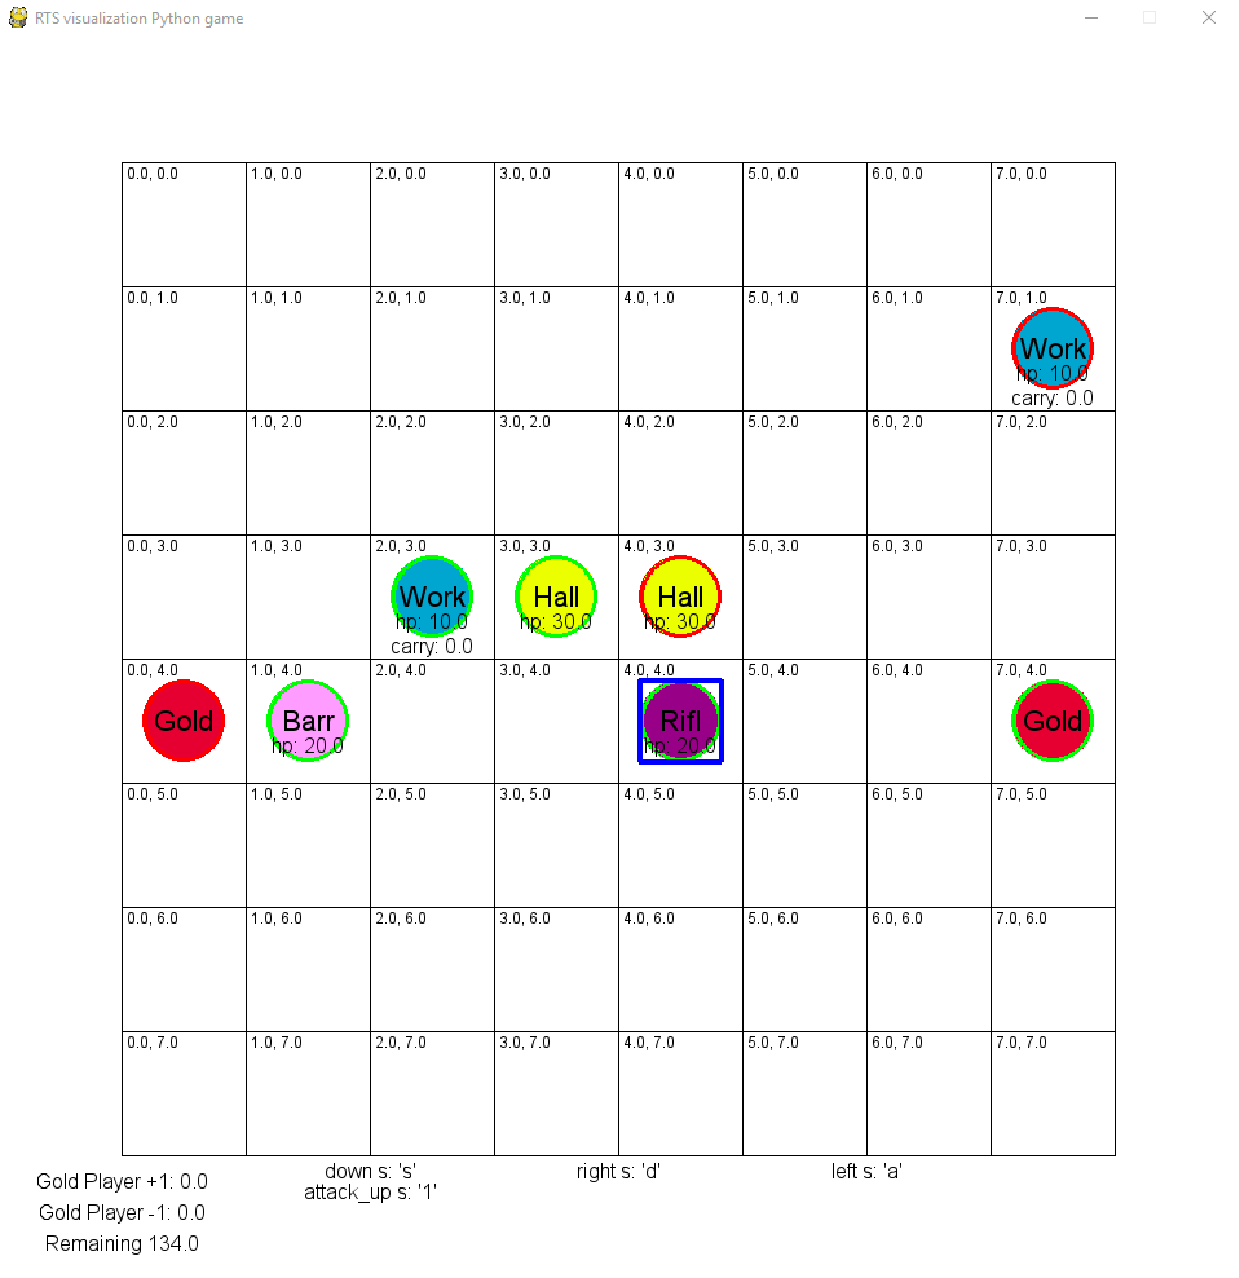
\includegraphics[width=0.8\textwidth]{photos/visualization_pygame.pdf}
	\end{center}
	\caption{Na zgornji sliki človeški igralec igra izgrajeno strateško igro proti računalniškim nasprotnikom.}
	\label{visualization_pygame}
\end{figure}

\section{Unreal Engine 4}
\label{UnrealEngine}

Celostni pogon Unreal Engine 4 (ang. game engine Unreal Engine 4; UE4) je odprto-kodni program podjetja Epic Games, ki je namenjen hitri izdelavi računalniških iger. 
Obstajajo drugi celostni pogoni kot je na primer Unity.\\
Unreal Engine 4 omogoča hitro ustvarjanje iger s pomočjo posebnih diagramov (ang. blueprint) in hkrati podpira programski jezik C++, ki ga uporabimo za hitro izvedbo velikega števila matematičnih izrazov~\cite{diploma2}.

\begin{figure}[h]
	\begin{center}
		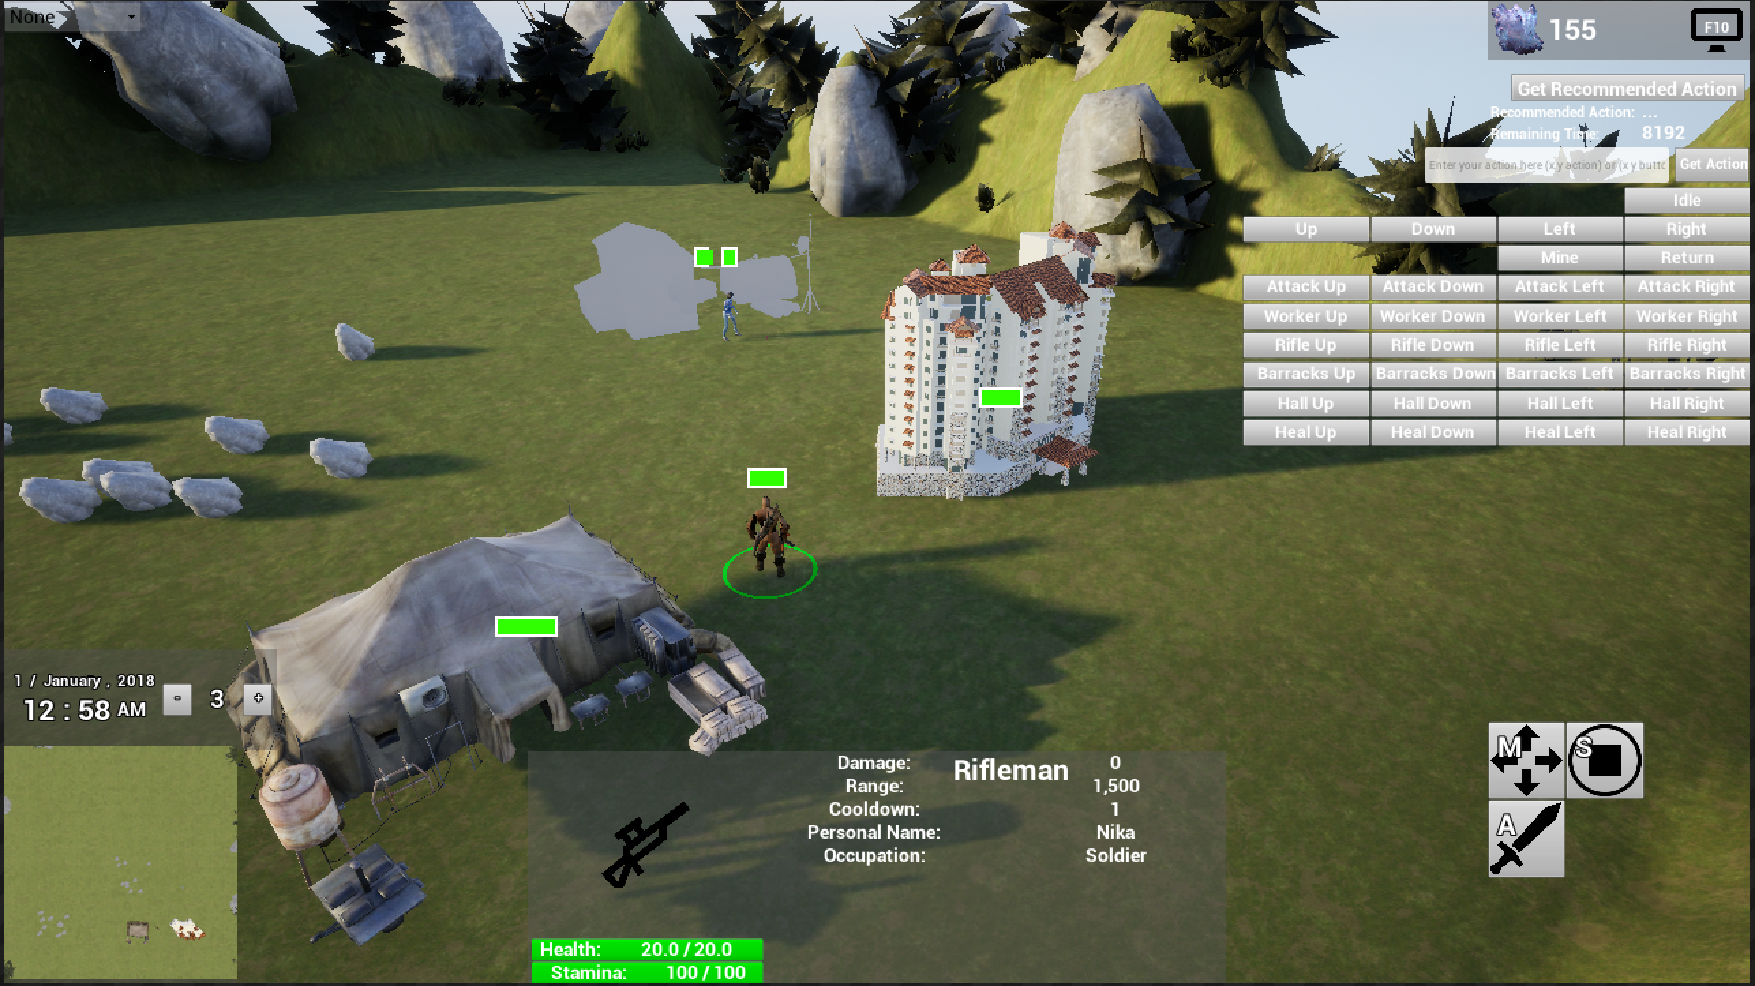
\includegraphics[width=0.8\textwidth]{photos/ue4-widget.pdf}
	\end{center}
	\caption{Zgornja slika predstavlja igro izdelano v Unreal Engine 4 z uporabniškim vmesnikom. Na sliki je vidna glavna hiša, vojašnica, vojak in delavec, kot tudi polje zlata na levi. Igralec lahko upravlja z vmesnikom za pošiljanje prošenj za predloge potez, ki je nakazan v vnosnim poljem in gumbi na desni strani slike. }
	\label{ue4-game}
\end{figure}

V temu programu smo oblikovali vizualizacijo igre, ki nam je omogočilo bolj moderen in realističen prikaz realno-časovne strateške igre, saj je vizualiziran seveda v 3-D in ne 2-D kot v Pygame.

V igri lahko izvajamo akcije preko uporabniškega vmesnika, kot tudi z bližnjicami na tipkovnici.
Kompleksnejši uporabniški vmesnik nam zagotavlja več funkcionalnosti kakor igra izdelana v Pygame.
Z njim lahko izbiramo več figur ter jih grupiramo v skupine.
Figuram postavljamo več zaporednih akcij, ki jih ta izvršuje v tem vrstnem redu.
Človeški igralec ima tudi vpogled na manjši zemljevid, prikazan v levem spodnjem kotu, na katerem vidi nasprotnikove in svoje figure.
Nekaj je tudi kozmetičnih funkcij kot na primer prekrivanje zemljevida z meglo (ang. Fog of war), dnevno-nočni cikel, animacije za vojskovanje, premikanje, nastavitve hitrosti časa ipd.
Igra ima tudi implementirana izvajalna drevesa, kjer na primer agentu naročimo nabiranje zlatnikov, ta jih sam vrača v najbližje odlagališče zlatnikov.
Izvajalna drevesa so implementirana tudi za napadanje, agentovo nedejavnost, kjer se agent prosto premika okrog, išče stavbe itd.
Igra ima implementirane tudi razne zvočne efekte, učinke delcev za prikaz zmanjšanja življenjskih točk nasprotnikovim enotam.
V igri lahko tudi stanje igre shranimo na disk in ga pozneje naložimo, da igro lahko igramo naprej.
Ob tem zapisovanju igre smo ugotovili pravi postopek, kako zajeti igro v Unreal Engine in ga zapisati v določen format, ki ga potem lahko lažje prenašamo.
To nam je koristilo tudi pri kodiranju igre v notacijo za označevanje JavaScript objektov (ang. JavaScript Object Notation; JSON), da smo jo lahko poslali kot parameter v zahtevku Python modulu.
Igra podpira tudi preprosto analitiko za primerjavo denarja med igralci, tipi figur ipd.

Igra je zasnovana tudi tako, da se lahko dva igralca med sabo pomerita preko mreže s spletnim podsistemom Steam ali preko lokalne mreže, preko katerega se lahko tudi komunicirata.
Oba igralca v tem primeru na svoji lokalnem računalniku poganjata naučena modela in od njega zahtevata priporočila akcij.
Ker lahko igralca izbereta več različnih map, na katerih bosta igrala, je potrebno za vsako izmed teh map naučiti svoj model, saj imajo lahko mape drugačne dimenzije v širini in višini.
Z zdajšnim algoritmom niso prokriti primeri, da določeno polje ni dosegljivo (voda, skalovje), tako da mape morajo biti kvadratne in vsa polja so dosegljiva.
Nekatere izmed zgoraj navedenih funkcij je izdelal Nick Pruehs v vtičniku ue4-rts~\cite{rtsUe4}, kot recimo nekej izvajalnih dreves, zemljevid, prekrivanje zemljevida z meglo.

Potrebno je bilo preslikati akcije in figure v urejevalnik Unreal Engine, da se tam figure primerno premikajo in izvajajo akcije.
Potrebno je bilo (mapirati) animacije, efekte, da premikanje in napadanje zgleda dokaj realistično.
Ko igralca pričneta z igranjem igre, se naloži TensorFlow model, katerega bosta igralca uporabljala za pridobivanje akcij.
Za lažjo komunikacijo z Python modulom in vračanje povratnih klicov v engine smo uporabili vtičnik tensorflow-ue4~\cite{ue4tf}, ki nadgradi vtičnik UnrealEnginePython~\cite{ue4python} s TensorFlow komponento. 
Ta komponenta se avtomatično naloži na odjemalčevem računalniku in zagotavlja, da lahko ta uporablja vse funkcionalnosti TensorFlowa.
 
Ko igralec ali računalniški nasprotnik poda zahtevo za pridobitev akcije, se prvo pridobi vse podatke o igri in se jih mapira v JSON zapis, da se ga potem pošlje Python skripti.
V tem JSON zapisu so zapisane figure s kodirniki (x, y, igralec ,tip figure, zdravje, nosi zlatnike ,zlatniki ,preostal čas).
Potem se seveda asinhrono pošlje Python skripti ta JSON zapis, ta izgradi novo šahovnico s figurami na podlagi prejetih zakodiranih figur.
Skripti se poda tudi ime igralca, ki zahteva akcijo.
Skripta za tem pokliče funkcijo za pridobitev verjetnosti akcij, ki izvede določeno število MCTS iteracij in izbere tisto z največjo verjetnostjo.
Python skripta vrne koordinati x in y ter akcijo, ki se potem ta izvede v celostnem pogonu s preslikanimi svojimi akcijami za gor, dol, napad, naberi ipd.
Potrebno je bilo tudi paziti z orientacijo koordinatnega sistema, saj je bil v Python igri drugače orientiran kot v pogonu Unreal Engine. 
Potrebno ga je bilo obrniti za -90° v osi Z (pogon Unreal Engine 4: +x gor, +y desno, Python igra: +x desno, +y dol)

Ta predstavitev omogoča tudi igranje dveh človeških igralcev enega proti drugemu preko internetne mreže, kjer vsak igralec pridobiva priporočene ukaze iz modela.
Človeški igralec lahko igra tudi proti računalniškim igralcem, ki vsake 0.5 sekund zahteva za novo najboljšo akcijo.
Lahko si tudi ogledamo dva računalniška igralca igrati drug proti drugemu.

\subsection{Prenos stanja igre}
Za vsakega od igralcev, se vzpostavi svoja komponenta za pridobivanje akcij, ki naloži model da je pripravljen na pridobivanje napovedi.
V trenutku lahko samo eden od igralcev pridobi napoved, saj pride do konfliktov, če se na primer oba igralca odločita figuro premakniti na isto polje.
Ko igralec pošlje prošnjo za napoved, zraven pošlje svoje stanje igre, in kateri igralec je tisti, ki pošilja prošnjo.
Na to algoritem nastavi trenutno igro na poslano in izbere najprimernejšo akcijo.
Po izvedbi izbrane akcije, igra počaka določen čas, da se akcija izvede do konca, za tem lahko ta postopek ponovi drugi igralec.

Človeški igralec lahko akcijo pridobi kadarkoli, a mora počakati da se trenutna prošnja za napoved konča. Za njim se postavi v čakalno vrsto tudi računalniški nasprotnik.
%%%%%%%%%%%%%%%%%%%%%%%%%%%%%%%%%%%%%%%%%%%%%%%%%%%%%%%%%%%%%%%%%%%%%%%%%%%%%%%%%%%%%%%%%%%%%%%%%%%%%%%%%%%%%%%%%%%%%%%%
%%%%%%%%%%%%%%%%%%%%%%%%%%%%%%%%%%%%%%%%%%%%%%%%%%%%%%%%%%%%%%%%%%%%%%%%%%%%%%%%%%%%%%%%%%%%%%%%%%%%%%%%%%%%%%%%%%%%%%%%
%%%%%%%%%%%%%%%%%%%%%%%%%%%%%%%%%%%%%%%%%%%%%%%%%%%%%%%%%%%%%%%%%%%%%%%%%%%%%%%%%%%%%%%%%%%%%%%%%%%%%%%%%%%%%%%%%%%%%%%%
%%%%%%%%%%%%%%%%%%%%%%%%%%%%%%%%%%%%%%%%%%%%%%%%%%%%%%%%%%%%%%%%%%%%%%%%%%%%%%%%%%%%%%%%%%%%%%%%%%%%%%%%%%%%%%%%%%%%%%%%
%%%%%%%%%%%%%%%%%%%%%%%%%%%%%%%%%%%%%%%%%%%%%%%%%%%%%%%%%%%%%%%%%%%%%%%%%%%%%%%%%%%%%%%%%%%%%%%%%%%%%%%%%%%%%%%%%%%%%%%%
\chapter{Rezultati}
\label{chrezultati}

V temu poglavju bomo predstavili več konfiguracij učenja in njihovih rezultatov v vizualizaciji Pygame.
Naučene modele, ki so med seboj kompatibilni, bomo med seboj primerjali in izpostavili, zakaj je zmagovalna konfiguracija boljša od poražene.
Za tem bomo naučen model povezali z pogonom Unreal Engine, kjer bosta dva računalniška nasprotnika igrala igro drug proti drugemu ter primer, kjer človeški igralec igra proti računalniškem igralcu ki uporablja naučen model za izbiro akcij.

Pri samem učenju smo uporabili  TensorFlow 1.9.0, Python 3.6 ter za vizualizacijo Pygame 1.9.4 in Unreal Engine 4.20.


\begin{table}
	
	\begin{center}
		
		\begin{tabular}{p{0.4\linewidth}|p{0.1\linewidth}|p{0.1\linewidth}|p{0.1\linewidth}|p{0.1\linewidth}}
			Tip konfiguracije                          & {\tt \ref{resultFirst}} & {\tt \ref{resultSecond}} & {\tt \ref{resultThird}} & {\tt \ref{resultFourth}}\\ \hline
			{\tt časovna omejitev}                     & 100                     & 200                      & 200                     & 200 / fn                \\
			{\tt iteracije}                            & 40                      & 20                       & 30 + 30                 & 20                      \\
			{\tt epizod}                               & 8                       & 8                        & 8                       & 8                       \\
			{\tt MCTS iskanj}                          & 50                      & 50                       & 30                      & 50                      \\
			{\tt primerjave}                           & 20                      & 20                       & 20                      & 20                      \\
			{\tt zgodovina učnih primerov}             & 8                       & 8                        & 8                       & 8                       \\
			{\tt epohi}                                & 100                     & 100                      & 100                     & 100                     \\
			{\tt začetni zlatniki}                     & 20                      & 20                       & 1                       & 1                       \\
			{\tt povečevanje zlatnikov}                & 5                       & 5                        & 1                       & 1                       \\
			{\tt zmanjšanje življenjskih točk}         & 20                      & 20                       & 20                      & 20                      \\
			{\tt količina zdravljenja}                 & 20                      & 20                       & 20                      & 20                      \\
			{\tt stroški zdravljenja}                  & 5                       & 5                        & 5                       & 5                       \\
			{\tt število polj}                         & 8 x 8                   & 8 x 8                    & 8 x 8                   & 6 x 6                   \\

		\end{tabular}
	\end{center}
	\caption{V tej tabeli so napisane konfiguracije definicij igre in učenja za spodaj opisane primere učenja modela.}
	\label{tabelLearnConfig}
\end{table}

Za učenje smo na voljo podali vse možne akcije.

\section{Učenje z ustavitveno funkcijo s časovno omejitvijo}
\label{resultFirst}
V prvi fazi smo poskusili učenje modela z manjšo časovno omejitvijo (100 potez) ter dovolj velikim številom iteracij tako da algoritem potrebuje kar nekaj časa, da dokonča z izvajanjem učenja.


\subsection{Numerično}

\begin{figure}[h]
	\begin{center}
		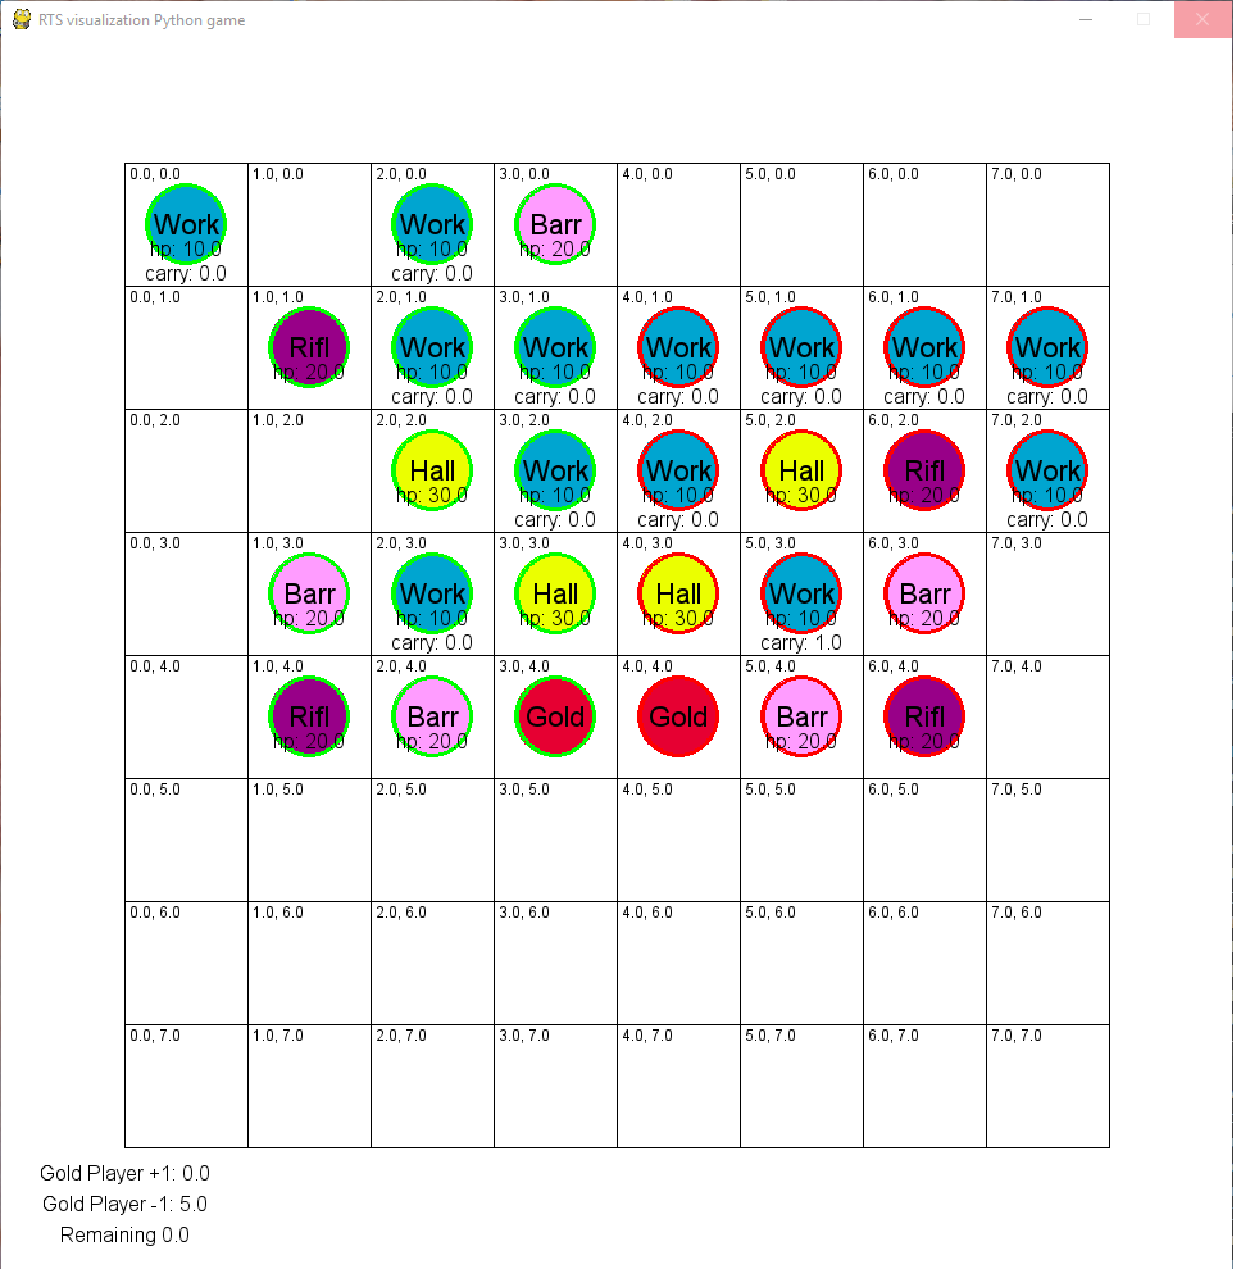
\includegraphics[width=0.6\textwidth]{photos/first-numeric.pdf}
	\end{center}
	\caption{Vizualizacija naučenega modela dveh računalniških nasprotnikov po izteku časovne omejitve v Pygame. Igralca sta se najbolj osredotočila na nabiranje zlatnikov in množični izgradnji cenejših figur.
		Uporabljen model je naučen z numeričnim kodirnikom. Učenje je potekalo 1 dan in 4 ure.}
	\label{vizualizacijaRezultatovNumericniKodirnik100Timeout}
\end{figure}


Numerični kodirnik se je bolj osredotočil na izdelavo delavcev, ki so najcenejše figure. 
Kar pomeni, da takoj ko je igralec imel dovolj denarja za izdelavo figure, jo je izdelal.
Igralca sta s svojimi figurami dobro nabirala zlatnike, s tem da sta glavna hiša in polje zlata neposredno drug ob drugem.

\subsection{Kodiranje z enico v zapisu vsakega stanja}

\begin{figure}[h]
	\begin{center}
		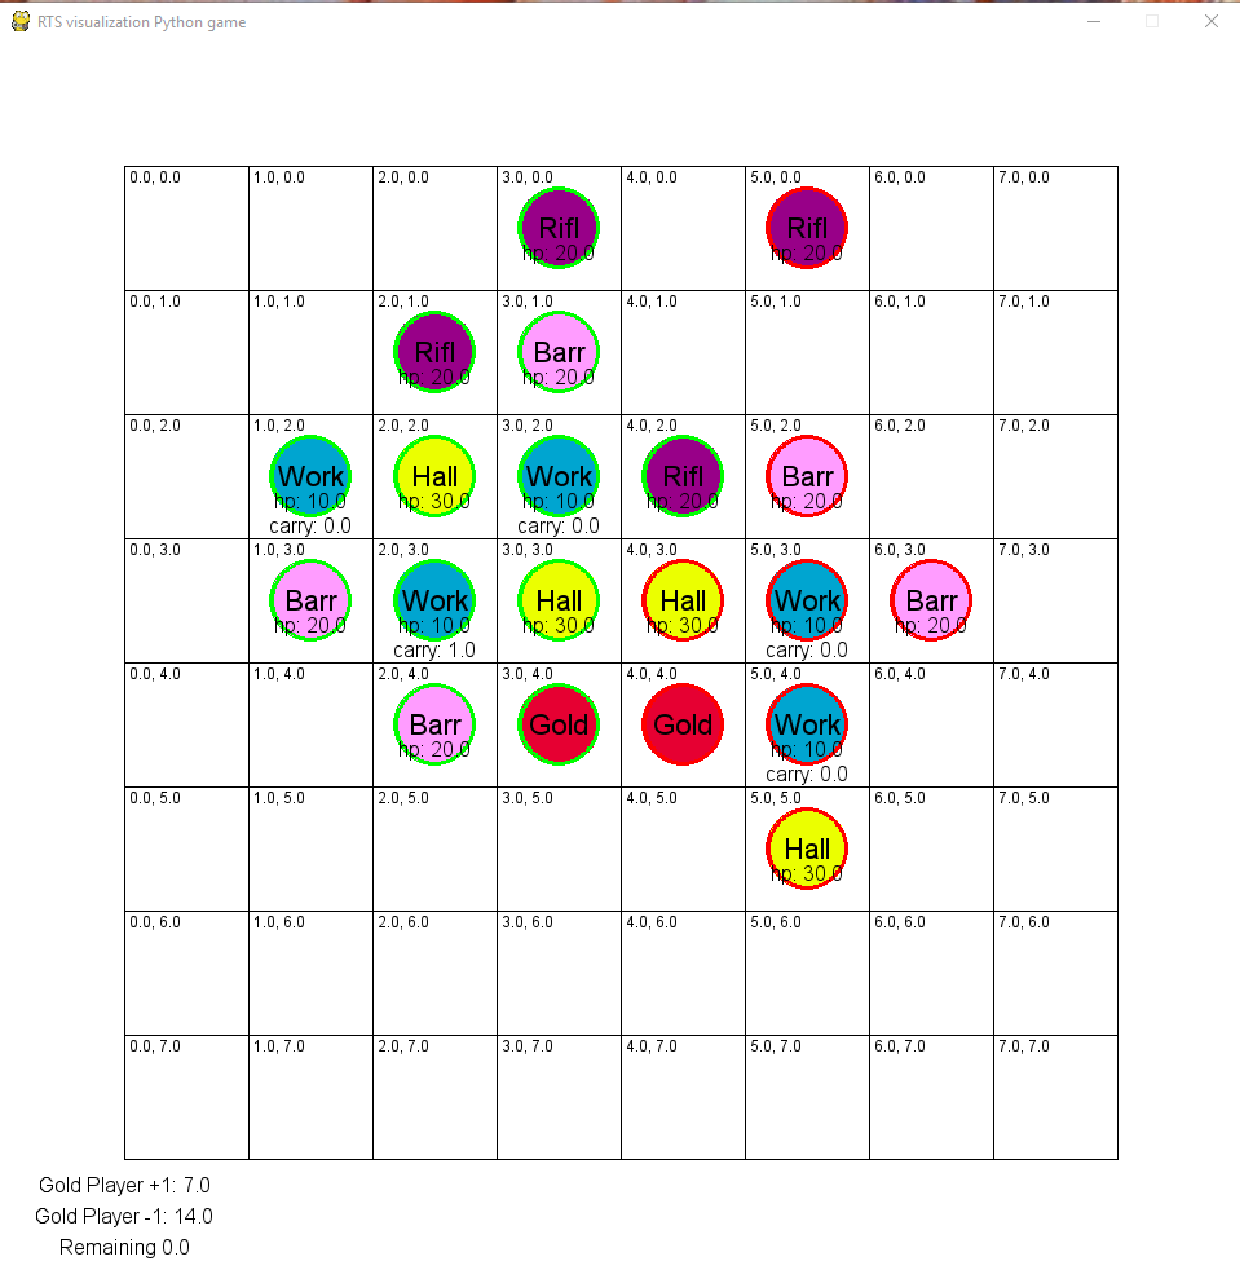
\includegraphics[width=0.6\textwidth]{photos/first-onehot.pdf}
	\end{center}
	\caption{Vizualizacija naučenega modela dveh računalniških nasprotnikov po izteku časovne omejitve v Pygame. Igralca sta se bolj osredotočala na izgradnjo vojaških figur ter napadanju sovražnih enot.
		Uporabljen model je naučen z one-hot kodirnikom. Učenje je potekalo 1 dan in 8 ur.}
	\label{vizualizacijaRezultatovOneHotKodirnik100Timeout}
\end{figure}

Z numeričnim kodiranjem se je algoritem osredotočil bolj na izdelavo vojaških figur in nabiranju samih zlatnikov.
Delavca sta stalno nabirala zlatnike in jih vračala v glavno hišo. 
Nabiranje in vračanje zlatnikov je v tem primeru veliko bolj konsistentno kakor z uporabno numeričnega kodirnika.
Igralca sta pozornost tudi deloma posvečala napadanju sovražnik figur, vendar ne do točke, kjer bi z napadanjem sovražnega igralca eliminirali.

\subsection{Primerjava}

Primerjali smo numerično kodiranje proti one-hot kodiranju na enakih konfiguracijah modelov ter igre.

Algoritem, naučen z one-hot kodiranjem ne more delovati pri primerjanju dveh modelov z numeričnim kodirnikom in obratno. 
Model učen z one-hot kodiranjem se lahko običajno pomerja samo proti drugemu modelu, ki je bil naučen z isto konfiguracijo.
Enako velja za numerični kodirnik.

Modele z različnimi konfiguracijami je med sabo težko primerjati, ne moreta igralca imeti različnih nastavitev za model, razen če jih eksplicitno prepišemo.
Primerjanje modelov smo prilagodili tako, da vsak izmed igralcev lahko uporablja drugačno konfiguracijo učnih parametrov~\ref{parametri}.
Za popolno primerjanje dveh različno naučenih modelov bi potrebovali tudi spremembe parametrov konfiguracije igre~\ref{chpravilaigre}, da bi lahko vsak izmed modelov deloval s poljubno konfiguracijo pravil igre, kot tudi tip ustavitvene funkcije ipd.
Ta sprememba bi preveč posegla v Surag Nairjevo različico algoritma AlphaZero, kar hočemo čim bolj ohraniti.

Izkazalo se je da one-hot kodiranje prinaša boljše rezultate po ocenitvi modelov z igranjem 20 iger drug proti drugemu, kjer je bil rezultat 20:0 za model zakodiran z one-hot načinom.

Algoritem je potrebno še predelati, tako da se lahko posameznem igralcu doda konfiguracijo pravil igre in učnih konfiguracij, kot tudi tip ustavitvene funkcije ipd.
S tem bi lahko primerjali dva popolnoma različna modela na isti konfiguraciji igre (npr šahovnica 8 x 8).

\section{Povečevanje časovne omejitve}
\label{resultSecond}
V tem koraku smo izbral kodirnih one-hot, ker se je v primerjavi pri prejšnji konfiguraciji obnesel boljše.

V tem primeru smo povečali časovno omejitev na 200 in znižali število iteracij na 20.
Povečali smo časovno omejitev, saj so se pri prejšni nastavitvi 100 igre prehitro zaključevale.
Znižali smo število iteracija na 20, saj bodo posamezne igre trajale dlje, in smo želeli približno isto časovno dolžino učenja, kot pri prejšnjem primeru, da lahko modela vsaj vizualno primerjamo.

\begin{figure}[h]
	\begin{center}
		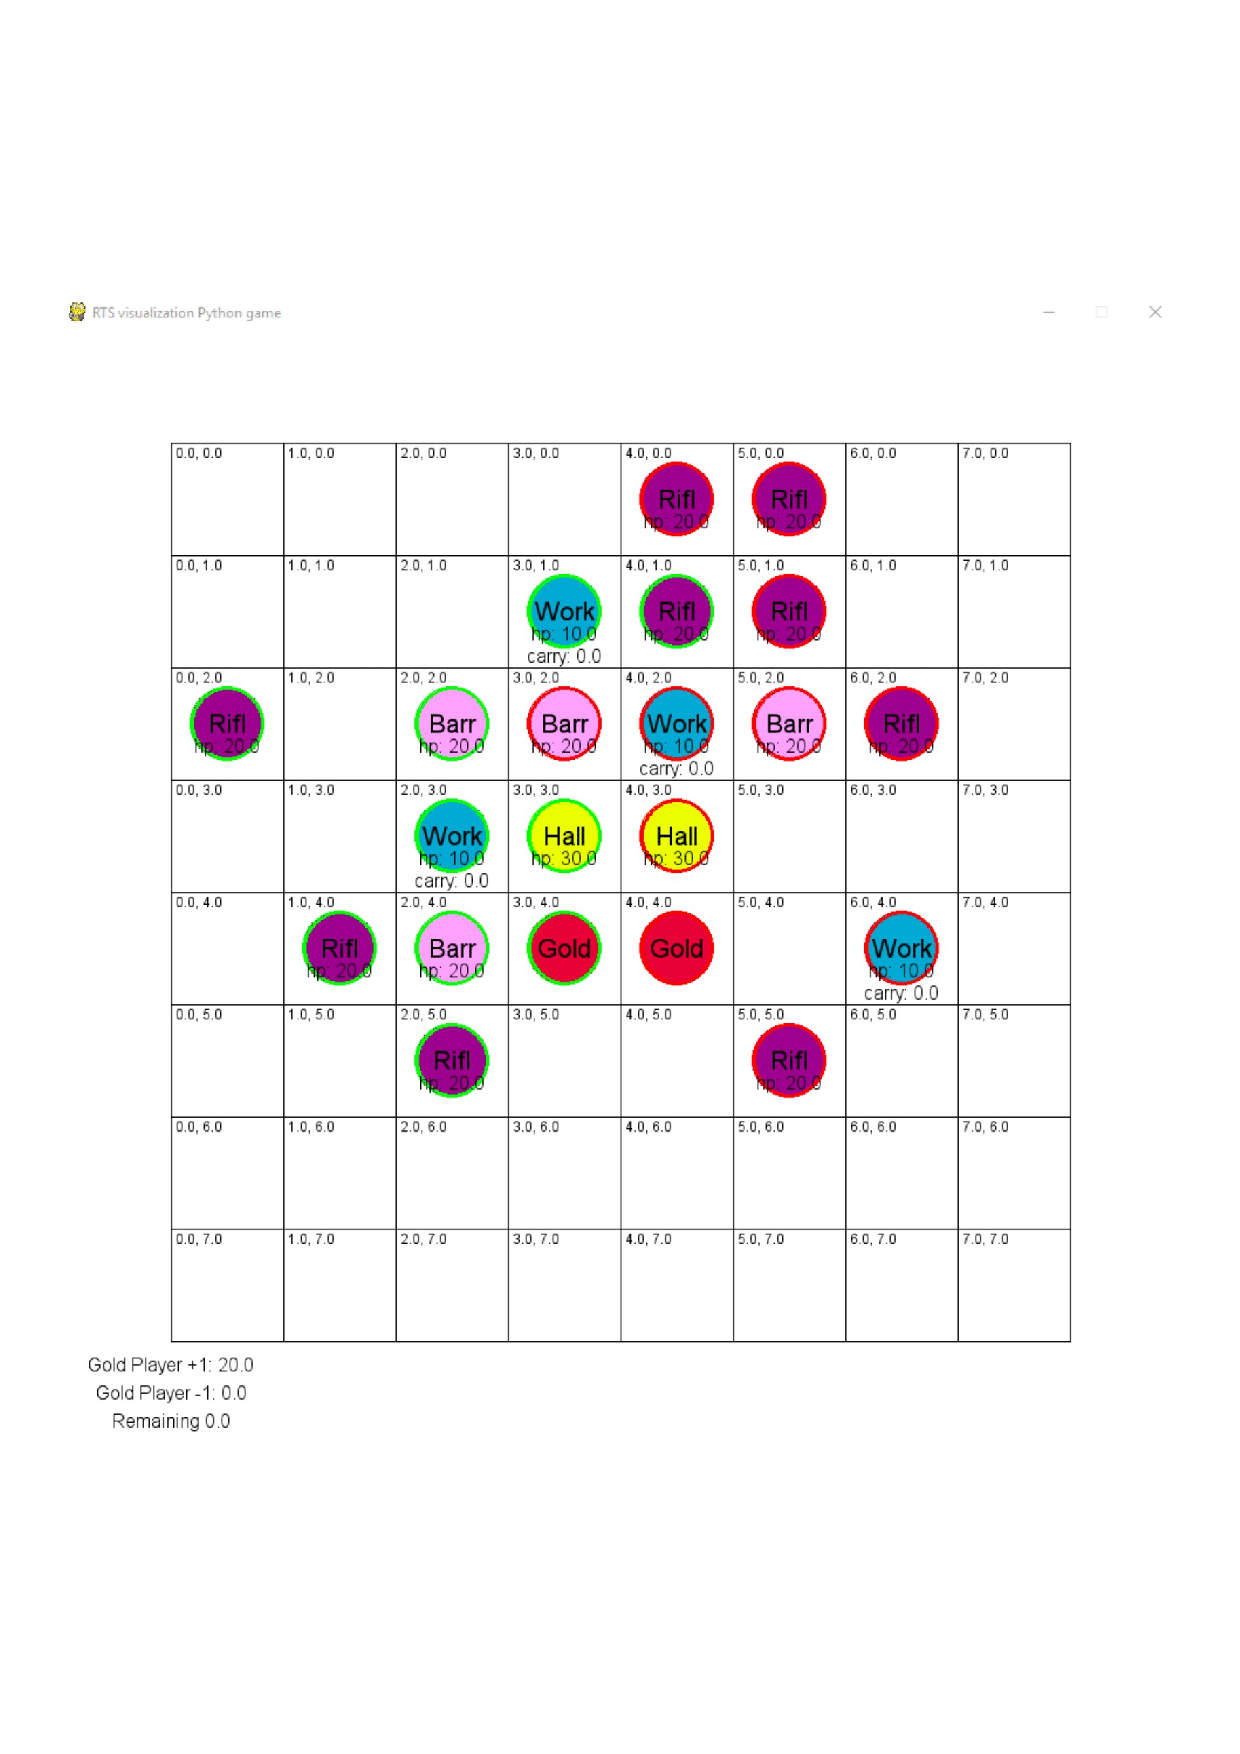
\includegraphics[width=0.6\textwidth]{photos/second-2018-11-12.pdf}
	\end{center}
	\caption{Vizualizacija naučenega modela v Pygame z povečano časovno omejitvijo  na 200 in znižano število iteracij na 20.}
	\label{vizualizacijaRezultatov200timeout20Iters}
\end{figure}

Algoritem se je bolj osredotočil na izdelavo vojaških figur in vojskovanja kot v prvi iteraciji učenja z manjšo časovno omejitvijo


\section{Sprememba konfiguracij zlata}
\label{resultThird}

Polji zlata smo pomaknil iz sredine na levi in desni rob, tako da se morajo delavci pomakniti do roba, nabrati zlatnike in jih vrniti nazaj v glavno hišo, ki je vedno na sredini mreže.
Spremenili smo nastavitev, koliko začetnih zlatnikov imata igralca iz 20 na 1, kar dovoli izgradnjo enega delavca na začetku igre.
Zmanjšali smo količino vrnjenega denarja iz 5 na 1, kar bi zagotavljalo, da morata igralca izbrati mnogo pravih sekvenc pomikanja do polja zlata, pridobiti zlatnike in jih vrniti v glavno hišo, preden bi lahko izgradili novo enoto.

\begin{figure}[h]
	\begin{center}
		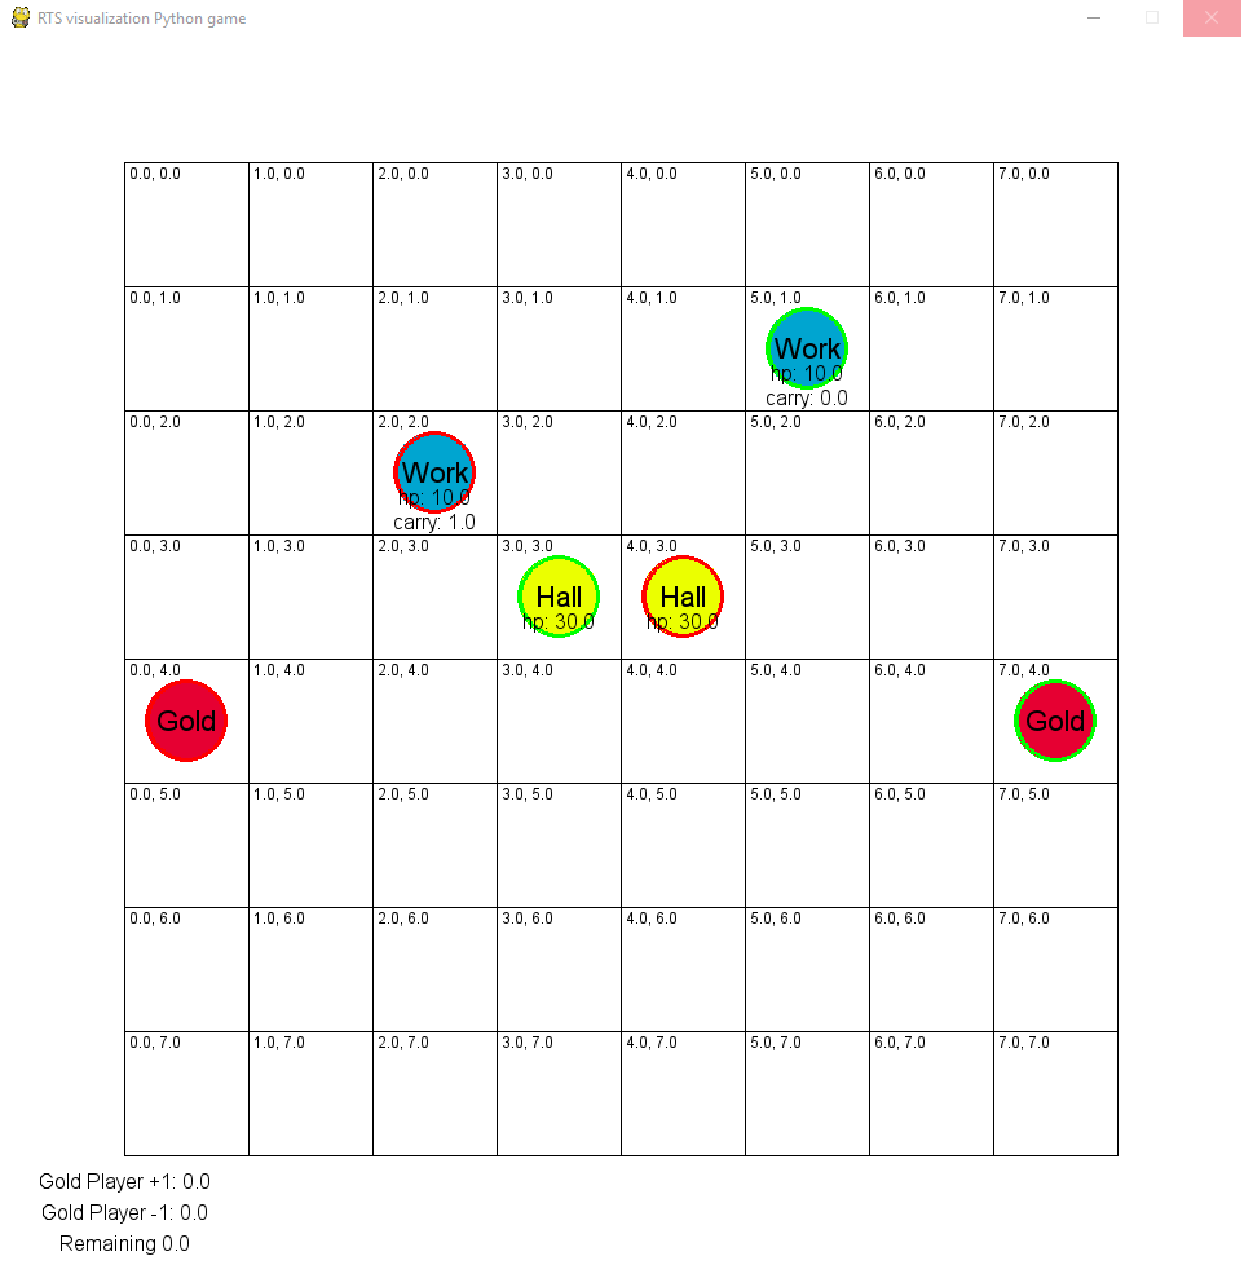
\includegraphics[width=0.6\textwidth]{photos/third-2018-11-14.pdf}
	\end{center}
	\caption{Vizualizacija naučenega modela v Pygame z polji zlata na robovih in glavnimi hišami v sredini. Delavci morajo hoditi daljšo razdaljo do polj zlata da iz njih naberejo zlatnike, ki jih za tem morajo vrniti v glavno hišo sredi šahovnice. }
	\label{vizualizacijaRezultatovSpremembaZlata}
\end{figure}

Model smo gradili 48 ur v dveh delih po 30 iteracij.
Prvi del učenja je potekal 24 ur in ni vračala nobenih koristnih rezultatov, saj sta se izurjena delavca samo sprehajala po šahovnici, brez da bi nabirala zlatnike.
Po nadaljevanju učenja obstoječega modela, ki je tudi potekal 24 ur smo pridobili boljše rezutate, ki vedno niso dobri.
Izurjena delavca sta tako kot prej skoraj naključno hodila po šahovnici, s tem da je kdo izmed njiju izvedel akcijo naberi zlatnike.
Zlatnikov potem ni vrnil do skoraj konca igre s časovno omejitvijo 200. Po vrnitvi zlatnikov je igralec takoj za tem izdelal dodatno enoto, kar je prineslo dovolj prednosti za zmago.
Zlatnike vrne v glavno hišo proti koncu iteracije igre. Mogoče algoritem čaka na konec igre, da preseneti nasprotnika, vendar bolj verjetno je da proti koncu igre MCTS začne bolj delovati, saj vrača prave vrednosti stanja igre, ki so končna stanja.
V tem primeru se je iz delovanja jasno razbralo, da MCTS ne vrača primernih rezultatov oziroma ne izboljša uteži modela dovolj dobro.
Dober primer je ta, da delavec hodi okrog glavne hiše z nabranimi zlatniki, vendar jih ne vrne v glavno hišo, kar bi povečalo njegov seštevek točk in se s tem postavil v prednost pred nasprotnikom.

S tem inkrementalnim učenjem modela v večih korakih smo prikazali, koliko počasi učenje te igre poteka in hkrati dokazali da se model izboljšuje.
Počasnost učenja je predvsem zaradi velikega števila akcij, ki se lahko na šahovnici pripetijo na vsakem polju.
Vseh možnih akcij je 30, kar privede v 8 x 8 x 30 = 1920 števil, ki jih prejme nevronska mreža kot vhodni nivo.
Zaradi števila akcij je počasno preverjanje katere izmed njih so veljavne, kar upočasni iteriranje stanj iger.

Tako kot smo opisali v sekciji poteku učenja~\ref{potekUcenja}, smo v tem primeru naleteli na težavo prekomernega prileganja, saj algoritem ni pravilno prepoznaval neodločene izide.
Neodločeni izidi niso bili kaznovani s strani primerjanja dveh modelov, pri katerih so se primerjale samo zmage in porazi novejšega modela proti starejšem.
Izidov je bilo skozi učenje vedno več neodločenih, pri katerem je pri 40. iteraciji učenja ostali samo neodločeni izidi, z redko zmago katerega izmed modelov in rezulta tega je bilo naključna hoja delavcev, s čimer so dosegli nov neodločen izid.
Popravek izbire modela je prinašal boljše rezultate, vendar je izbira novejšega modela veliko težja, saj dobra algoritma velikokrat dosežeta neodločen izid, posebej v začetnih stopnjah igre, kjer imata oba igralca malo zlatnikov in figur.
\section{Zmanjševanje velikosti šahovnice}
\label{resultFourth}

V tej konfiguraciji učenja smo zmanjšali velikost šahovnice iz 8 x 8 na 6 x 6.
Zmanjšali smo tudi število iteracij iz 30 na 20, saj bi teoretično bilo potrebnih manj iteracij za učenje manjše šahovnice.

Zmanjševanje šahovnice je privedlo do pričakovanih rezultatov.
Igralca sta občasno nabirala zlatnike, saj je polje zlatnikov v bližini glavne hiše, tako da se delavec postavi med glavno hišo in zlatnike in jih nabira brez da bi se moral premakniti.
Zaradi nabranih zlatnikov potem igralca izdelata nove delavce.

Število nabranih zlatnikov in izdelanih delavcev je vedno majhno.

\subsection{Ustavitvena funkcija zmanjšanja življenjskih točk}

V tem primeru smo uporabili ustavitveno funkcijo, ki zmanjšuje število življenjskih točk figuram, opisano v sekciji~\ref{sKillFunction}.
Po določenem številu potez (v našem primeru 90) funkcija prične izmenično zmanjševati življenjske točke igralčevih enot.

Uporaba funkcije v primerjavi z ustavitvenim časom je proizvedla slabše rezultate.
Igralca nabereta manj zlatnikov in posledično izdelata manj figur.

\begin{figure}[h]
	\begin{center}
		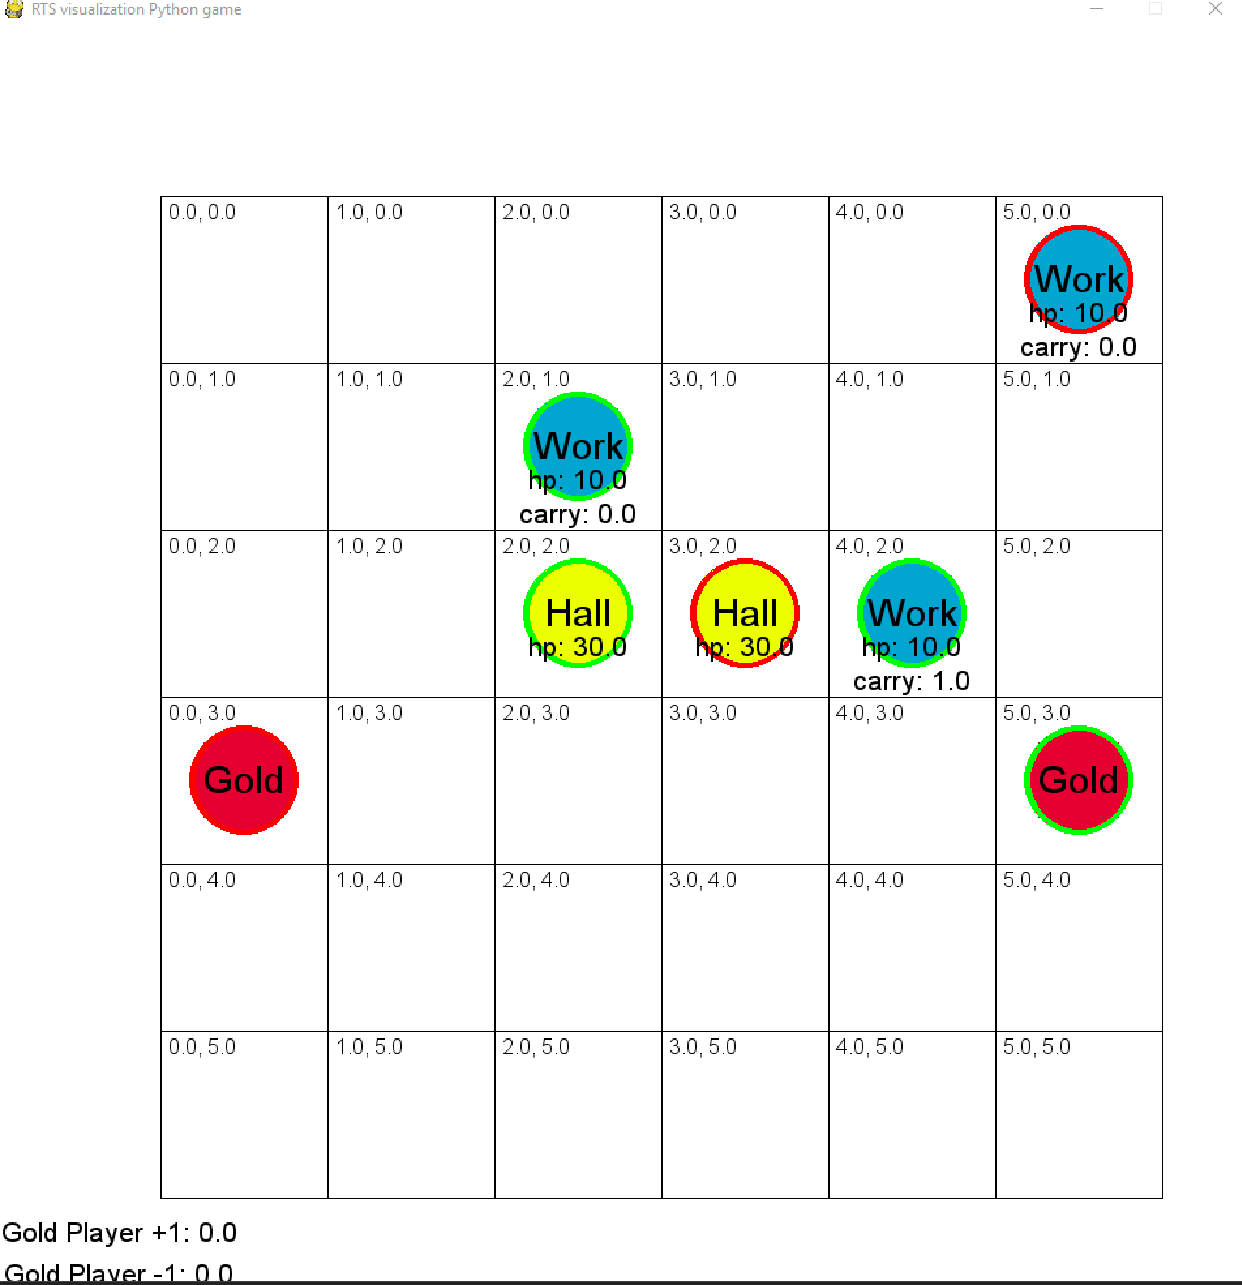
\includegraphics[width=0.8\textwidth]{photos/killFunction.pdf}
	\end{center}
	\caption{Zgornja slika prikazuje stanje igre pri 70. potezi, ki je naučena z uporabo ustavitvene funkcije zmanjšanja življenjskih točk. 
		Igralca sta nabirala zlatnike, in izurila nova delavca, vendar je postopek potekal slabše kakor brez te ustavitvene funkcije. }
	\label{vizualizacijaRezultatovKillFunction}
\end{figure}

Ta način učenja modela ni primeren, saj ni popolnoma kompatibilen z običajnimi RTS igrami, saj se igralčevim enotam življenjske točke ne odštevajo zaradi neznanega razloga.
Možno bi bilo ta način učenja aplicirati v igre, kjer nekatere izmed figur lahko prejmejo znižanje življenjskih točk zaradi naravnih dejavnikov, kot npr. mraz, strupen plin ipd.

\section{Vizualizacija rezultatov v pogonu Unreal Engine}
Proti koncu smo rezultate vizualizirali v pogonu Unreal Engine 4, ki ga je izdelalo podjetje Epic Games.
Izbiranje potez deluje izmenjujoče z zamikom pol sekunde, da se akcije končajo, preden se pošlje nov zahtevek z novim kodiranjem stanja igre.

\begin{figure}[h]
	\begin{center}
		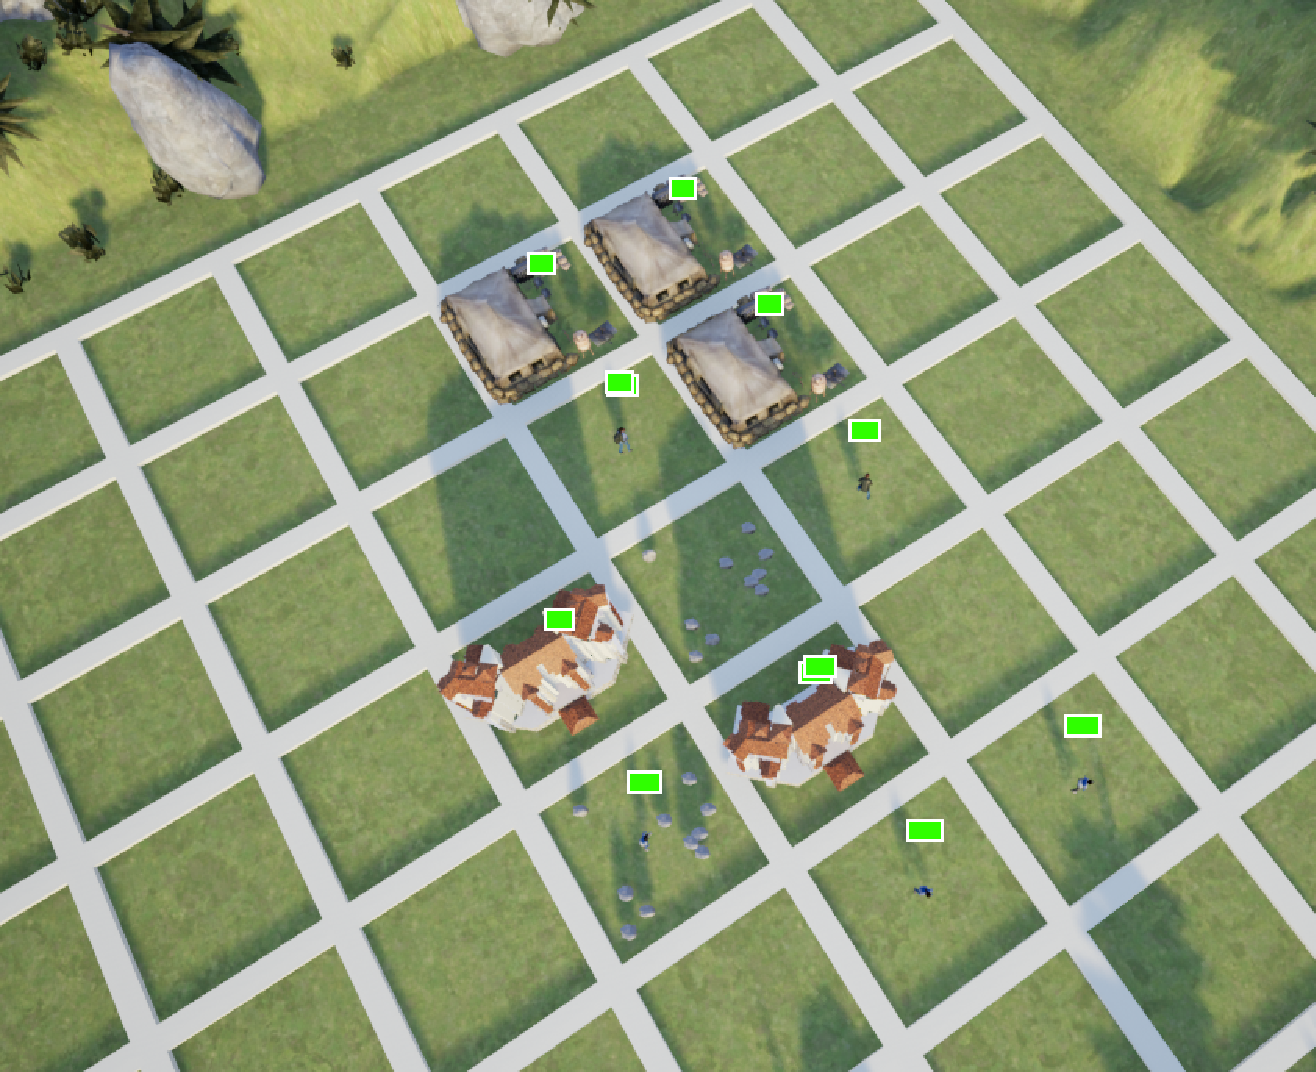
\includegraphics[width=0.8\textwidth]{photos/visualization_ue4.pdf}
	\end{center}
	\caption{Zgornja slika predstavlja igranje igre dveh računalniških nasprotnikov enega proti drugemu. V sredini vidimo glavni hiši in polja zlata, okrog vojašnice in delavce. }
	\label{visualization_ue4}
\end{figure}

Igranje proti računalniškem nasprotniku je z uporabo tega algoritma možno, vendar je nasprotnik prelahek, da bi bil primeren za njegovo aplikacijo v modernejše strateške igre.

%%%%%%%%%%%%%%%%%%%%%%%%%%%%%%%%%%%%%%%%%%%%%%%%%%%%%%%%%%%%%%%%%%%%%%%%%%%%%%%%%%%%%%%%%%%%%%%%%%%%%%%%%%%%%%%%%%%%%%%%
%%%%%%%%%%%%%%%%%%%%%%%%%%%%%%%%%%%%%%%%%%%%%%%%%%%%%%%%%%%%%%%%%%%%%%%%%%%%%%%%%%%%%%%%%%%%%%%%%%%%%%%%%%%%%%%%%%%%%%%%
%%%%%%%%%%%%%%%%%%%%%%%%%%%%%%%%%%%%%%%%%%%%%%%%%%%%%%%%%%%%%%%%%%%%%%%%%%%%%%%%%%%%%%%%%%%%%%%%%%%%%%%%%%%%%%%%%%%%%%%%
%%%%%%%%%%%%%%%%%%%%%%%%%%%%%%%%%%%%%%%%%%%%%%%%%%%%%%%%%%%%%%%%%%%%%%%%%%%%%%%%%%%%%%%%%%%%%%%%%%%%%%%%%%%%%%%%%%%%%%%%
%%%%%%%%%%%%%%%%%%%%%%%%%%%%%%%%%%%%%%%%%%%%%%%%%%%%%%%%%%%%%%%%%%%%%%%%%%%%%%%%%%%%%%%%%%%%%%%%%%%%%%%%%%%%%%%%%%%%%%%%

\chapter{Diskusija}
\label{chdiskusija}

Kot smo v poglavju~\ref{chrezultati} ugotovili, učenje modela poteka zelo počasi, vendar se model uspešno uči.
Zasnova opisa igre in njenega kodiranja je prava, ker učenje poteka uspešno.
Poteka počasi zaradi ustavitvenega pogoja in ocenitvenih funkcij, ki ugotovi zmagovalca ob tem ustavitvenem pogoju, ki mogoče ni pravi zmagovalec ob koncu igre.
MCTS naredi zelo majhno število iskanj in ne simulira igre do konca oziroma določene globine, kjer bi ugotovil stanje igre ter to stanje vrnil nazaj, ampak stanje igre pridobi od naučenega modela, ki velikokrat ni pravo.



V sklopu te diplomske naloge se nismo podajali v spreminjanje zgradbe nevronske mreže, temveč smo vzeli že izgrajeno nevronsko mrežo, primerno za učenje igre Othello.
Mogoče bi ravno sprememba strukture nevronske mreže privedla do boljših rezultatov, saj je matrika stanja igre veliko globja, kakor pri igri Othello.

Pri opisu igre je veliko problemov povzročalo uravnovešanje parametrov igre, kot na primer število vrnjenih zlatnikov, količina in cena zdravljenja ipd.
Dober primer neuravnovešene konfiguracije igre sta bila prav količina in cena zdravljenja, kjer je stalno samo nabiral zlatnike in zdravil svoje figure, tako da je dosegal vedno daljše število narejenih potez.
Zaradi tega je učenje potekalo zelo počasi, saj so posamezne igre trajale predolgo da so se zaključile.
Največ problemov je pri opisu igre povzročal ustavitveni pogoj.
Ocenitev stanja igre ni najboljša, saj je pridobljena po preprosti formuli, ki seveda ne vključuje vse dejavnike igre.



Algoritem se da dobro aplicirati v pogon Unreal Engine z nekaj vtičniki, opisanimi v razdelku~\ref{UnrealEngine}. Več igralcev lahko na istem računalniku zahteva priporočila akcij. 
Če igra poteka preko mreže, vsak igralec na svojem računalniku poganja algoritem, ki ne ovira delovanje drugih TensorFlow sej na računalnikih drugih igralcev.
Sama igra, napisana v programskem jeziku Python, na kateri je bil naučen model se ne preslika direktno v dejansko igro napisano v Unreal Engine.
V tej igri se akcije ne zgodijo takoj ob izvršitvi ukaza, saj vojaške enote in delavci potrebujejo nekaj časa da se premaknejo na drugo lokacijo, izvedejo akcijo kot na primer nabiranje zlatnikov, ki se tudi ne izvede takoj.
Zaradi trajanja akcij, asinhronosti pridobivanja priporočila, ki jih vrača Python modul, se lahko zgodi, da stanje igre ni več takšno, kakršno je bilo pri pošiljanju zahtevka za priporočilo, in bi bila priporočena akcija z asinhrono skripto drugačna. 
V nekaterih primerih se ob takih pogojih dve figuri premakneta na isto polje, oziroma izgradi stavba na polju, kjer je trenutno enota. 
Rešitev za je vpeljava zahtevanja priporočil akcij ko so akcije zaključene, ter nezmožnost izvajanja akcij v času od zahtevka priporočila do vrnjenega rezultata.
Ta rešitev je primerna za strateške igre, vendar ne za podkategorijo realno-časovnih strateških iger, ki pa zahtevajo takojšno napoved akcije.

Naučen model vrača samo 1 akcijo, ki ne more vključevati večjo skupino figur, kot na primer vseh vojaških enot, da se premaknejo proti nasprotnikoviku za napad.
Večino teh akcij so tudi omejene na sosednja polja, kot na primer pomik gor, dol, napad gor ipd., kar tudi ni primerna aplikacija v dejansko igro, kjer se lahko figure premikajo v poljubnih dolžinah in smereh.
%%%%%%%%%%%%%%%%%%%%%%%%%%%%%%%%%%%%%%%%%%%%%%%%%%%%%%%%%%%%%%%%%%%%%%%%%%%%%%%%%%%%%%%%%%%%%%%%%%%%%%%%%%%%%%%%%%%%%%%%
%%%%%%%%%%%%%%%%%%%%%%%%%%%%%%%%%%%%%%%%%%%%%%%%%%%%%%%%%%%%%%%%%%%%%%%%%%%%%%%%%%%%%%%%%%%%%%%%%%%%%%%%%%%%%%%%%%%%%%%%
%%%%%%%%%%%%%%%%%%%%%%%%%%%%%%%%%%%%%%%%%%%%%%%%%%%%%%%%%%%%%%%%%%%%%%%%%%%%%%%%%%%%%%%%%%%%%%%%%%%%%%%%%%%%%%%%%%%%%%%%
%%%%%%%%%%%%%%%%%%%%%%%%%%%%%%%%%%%%%%%%%%%%%%%%%%%%%%%%%%%%%%%%%%%%%%%%%%%%%%%%%%%%%%%%%%%%%%%%%%%%%%%%%%%%%%%%%%%%%%%%
%%%%%%%%%%%%%%%%%%%%%%%%%%%%%%%%%%%%%%%%%%%%%%%%%%%%%%%%%%%%%%%%%%%%%%%%%%%%%%%%%%%%%%%%%%%%%%%%%%%%%%%%%%%%%%%%%%%%%%%%

\chapter{Zaključek}
\label{chzakljucek}
V diplomski nalogi smo povzeli kaj realno-časovna strateška igra je, da smo jo lahko uspešno tudi implementirali.
Pregledali smo njihove nivoje nadzorovanja in abstrakcije in s kakšnega zornega kota na njih gledajo nevronske mreže.
Za tem smo se podali v raziskovanje algoritmov za učenje te strateške igre in smo naleteli na algoritem AlphaZero.
Na hitro smo pregledali njegovo zgodovino in korake k samostojnem algoritmu, ki je primeren za reševanje poljubne igre z metodami samoučenja.
Ta algoritem smo potem podrobneje pregledali, da smo njegov proces učenja in igranja iger razumeli, da smo lahko za tem opisali svojo strateško igro v jeziku Pythonu.
Določili smo pravila igre in glavne cilje, ki jih strateška igra mora imeti.
Pri tem smo morali paziti da smo se držali okvira Surag-Nairjeve implementacije algoritma AlphaZero, da smo lahko zanj pripravili svojo strateško igro, ki je kompatibilna z njegovim algoritmom.
Za tem smo določili akcije ki jih figure lahko izvajajo in jih abstrahirali, tako da so za algoritem nedvoumne in hitre.
Da smo nevronski mreži lahko podali stanje igre, smo ga morali pravilno zakodirati.
Izbrali smo desetiški in one-hot način kodiranja, med katerima se je one-hot izkazal uspešnejši, saj v prednost ne postavlja večjih zakodiranih števil kot boljših.
Za tem smo ugotovili pravšnji način evalvacije stanja igre in njen ustavitveni pogoj.
Določili smo ustavitveno ranjujočo funkcijo, ki dovoljuje bolj aktivnim igralcem daljše igranje, vendar jih kaznuje iz razlogov, ki sami strateški igri niso naravni.
Drugi pristop ustavitvenega pogoja je bil časovni iztek, pri katerem se je po določenem številu potez presodilo, kateri igralec je zmagovalen po določenem kriteriju.
Ko smo imeli opisano igro, smo morali ugotoviti primerne nastavitve in jih uporabiti pri samem učenju igre in izbrati parametre.
Za tem smo pripravili vizualizacijo igre v jeziku Python z modulom Pygame, ki prikaže igro v preprosti šahovnici in figure s krogci.
V pogonu Unreal Engine 4 smo pripravili bolj kompleksno strateško igro, ki je boljša predstavitev dejanske realno-časovne strateške igre.
V tej igri pošiljamo zahtevke za akcije preko vtičnika v Python skripto, v katero podamo trenutno stanje igre, nazaj dobimo priporočeno akcijo.
Zahtevke lahko pošilja računalniški nasprotnik ali človeški igralec, ko v najboljšo akcijo ni prepričan.
Za tem smo se posvetili predvsem učenju modelov z različnimi konfiguracijami ter jih vizualizirali v Pygame in Unreal Engine.
Ugotovili smo, da je učenje počasnejše zaradi kompleksnosti igre in načina zgradbe nevronske mreže, vendar poteka uspešno, s tem da ne daje večjo prednost igralcu 1 kot -1 ipd.
Diplomska naloga je dober prispeve k Surag-Nairjevim igram za AlphaZero, ki razširi preproste igre črno-belih figur v figure večih atributov.
V to igro smo pripeljali tudi časovne kompleksnosti in jo razširili z vizualizacijo v Pygame in Unreal Engine 4.

Igro, izdelano v UE4~\cite{td2020} in AlphaZero General algoritem s Pygame igro~\cite{pygameAlphaZeroGeneral} smo dodali na spletno gostovanje GitHub pod odprto licenco.

\newpage %dodaj po potrebi, da bo številka strani za Literaturo v Kazalu pravilna!
\ \\
\clearpage
\addcontentsline{toc}{chapter}{Literatura}
\bibliographystyle{plain}
\bibliography{literatura}


\end{document}

